\chapter{Theoretical Basis for CFAST}

Adequately detailed documentation of the theoretical basis of the model allows the model user to
understand the underlying theory behind the model implementation and thus be able to assess the
appropriateness of the model to specific problems. This chapter presents a derivation of the
predictive equations for zone fire models and explains in detail the ones used in CFAST.

The modeling equations used in CFAST take the mathematical form of an initial value problem
for a system of ordinary differential equations. These equations are derived using the
conservation of mass, the conservation of energy (equivalently the first law of thermodynamics),
the ideal gas law. These equations predict as functions of time quantities such as pressure, layer
height and temperatures given the accumulation of mass and enthalpy in the two layers. The
assumption of a zone model is that properties such as temperature can be approximated
throughout a control volume by an average value.

Many formulations based upon these assumptions can be derived. One formulation can be
converted into another using the definitions of density, internal energy and the ideal gas law.
Though equivalent analytically, these formulations differ in their numerical properties. Each
formulation can be expressed in terms of mass and enthalpy flow. These rates represent the
exchange of mass and enthalpy between zones due to physical phenomena such as plumes,
natural and forced ventilation, convective and radiative heat transfer, and so on. For example, a
vent exchanges mass and enthalpy between zones in connected rooms, a fire plume typically
adds heat to the upper layer and transfers entrained mass and enthalpy from the lower to the
upper layer, and convection transfers enthalpy from the gas layers to the surrounding walls.

As discussed in references \cite{Forney:1994} and \cite{Rehm:1992}, the zone fire modeling ordinary differential equations (ODEs) are stiff. The term stiff means that large variations in time scales are present in the ODE solution. In our problem, pressures adjust to changing conditions more quickly than other to solve zone fire modeling ODEs because of this stiffness. Runge-Kutta methods or predictor-corrector methods such as Adams-Bashforth require prohibitively small time steps in order to
track the short-time scale phenomena (pressure in our case). Methods that calculate the Jacobian
(or at least approximate it) have a much larger stability region for stiff problems and are thus
more successful at their solution.

\section{Derivation of Equations for a Two-Layer Model}

A compartment is divided into two control volumes, a relatively hot upper layer and a relatively cool lower layer, as illustrated in figure \ref{fig:Control_Volumes}.  The gas in each layer has attributes of mass, internal energy, density, temperature, and volume denoted respectively by $m_i$, $E_i$, $\rho_i$, $T_i$, and $V_i$ where $i$=$L$ for the lower layer and $i$=$U$ for the upper layer.  The compartment as a whole has the attribute of pressure $P$.  These 11 variables are related by means of the following seven constraints (counting density, internal energy and the ideal gas law twice, once for each layer).

\be \rho _i  = \frac{{m_i }}{{V_i }} {\hspace{1.0in} \textnormal{Density}} \label{eq:density} \ee

\be  E_i = c_v m_i T_i {\hspace{1.0in} \textnormal{Internal Energy}} \label{eq:internal_energy} \ee

\be P = R\rho _i T_i {\hspace{1.0in} \textnormal{Ideal Gas Law}} \ee

\be V = V_L + V_U {\hspace{1.0in} \textnormal{Total Volume}} \label{eq:volume} \ee

\begin{figure}[h]
\begin{center}
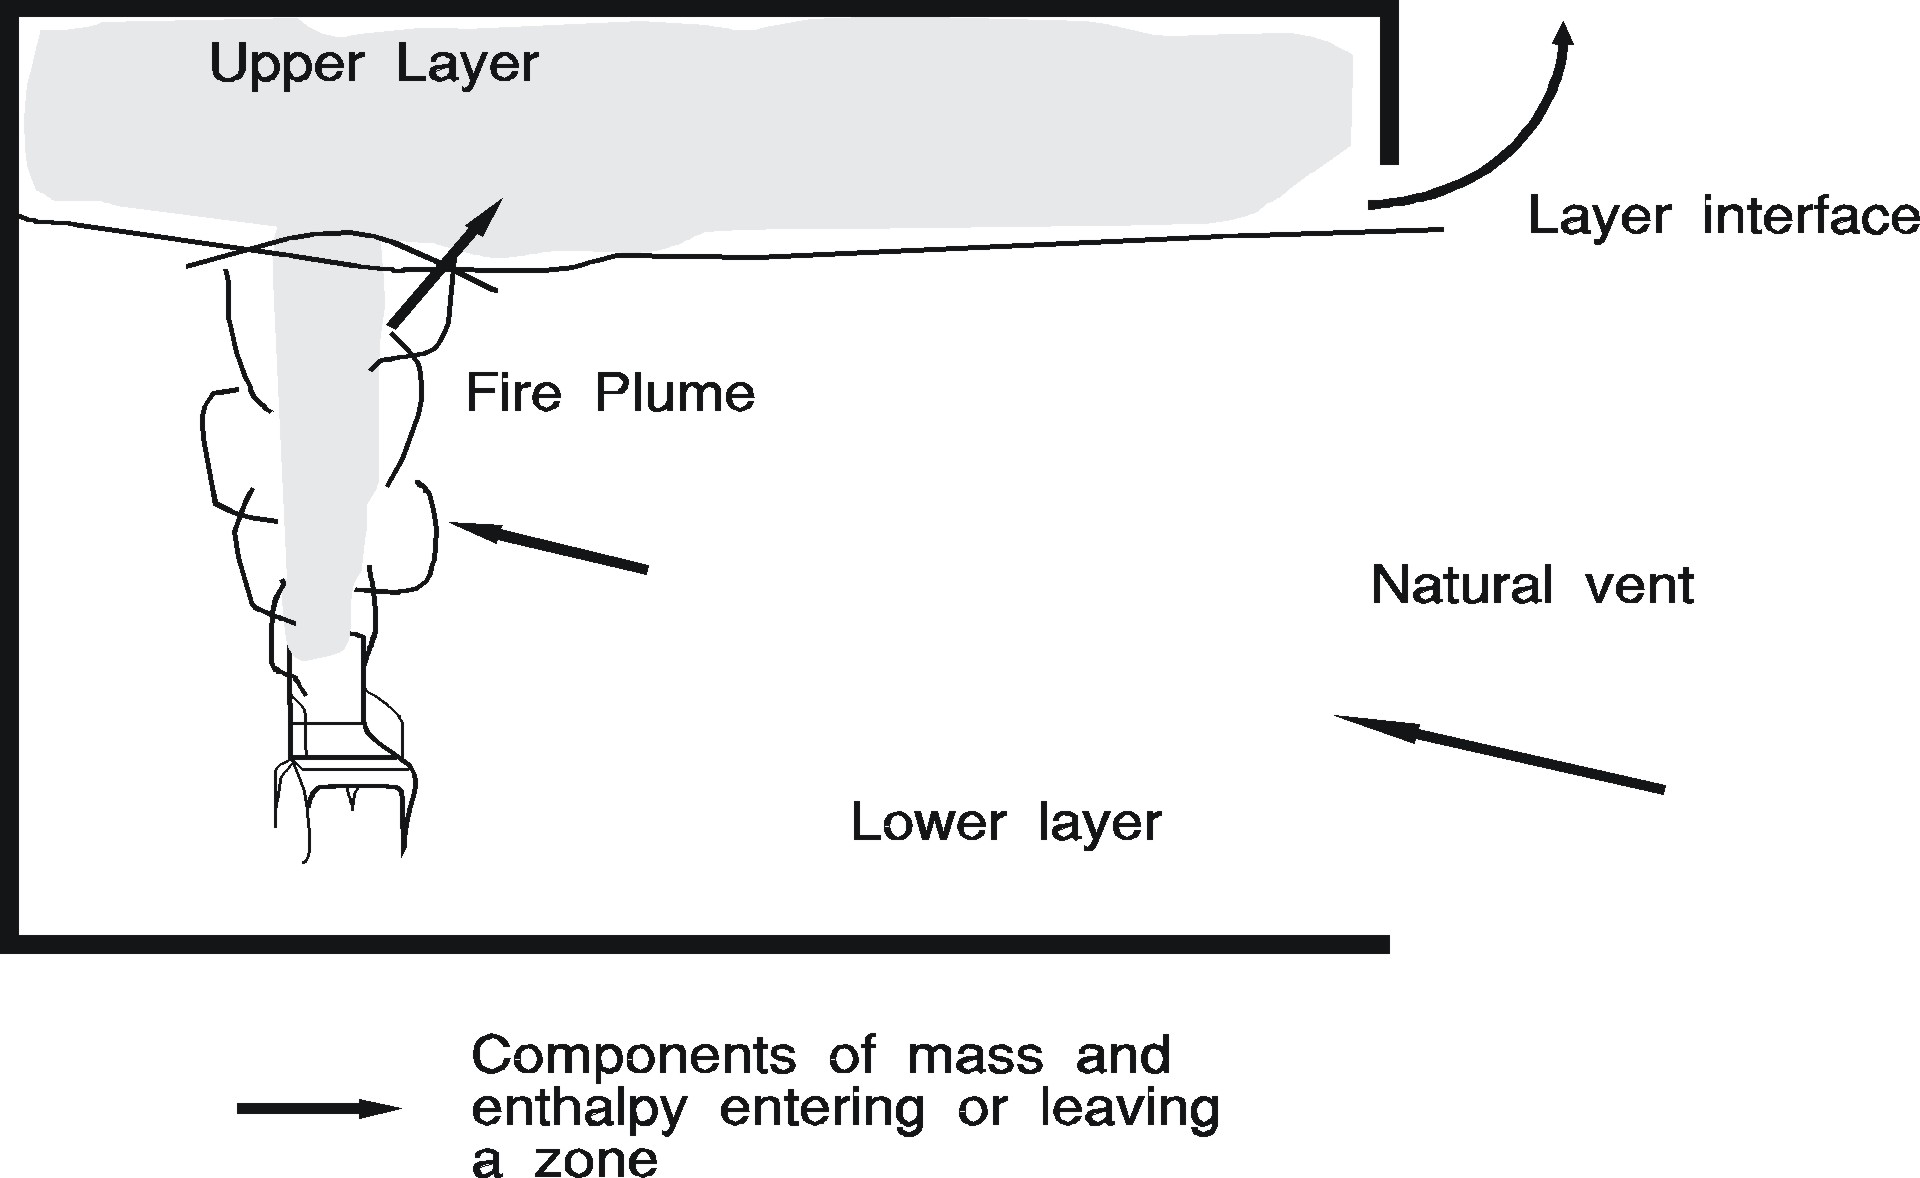
\includegraphics[width=5.0in]{FIGURES/Theory/Control_Volumes}\\
\end{center}
\caption{Schematic of control volumes in a two-layer zone model.}
 \label{fig:Control_Volumes}
\end{figure}

The specific heat at constant volume and at constant pressure $c_v$ and cp, the universal gas constant, R, and the ratio of specific heats, $\gamma$, are related by $\gamma = c_p / c_v$ and $R = c_p- c_v$.  For ambient air, $c_p \approx 1$ kJ/kg K and $\gamma = 1.4$.  Four additional equations obtained from conservation of mass and energy for each layer are required to complete the equation set.  The differential equations for mass in each layer are 

\be \frac{{dm_L }}{{dt}} = \dot m_L \ee

\be \frac{{dm_U }}{{dt}} = \dot m_U \ee

The first law of thermodynamics states that the rate of increase of internal energy plus the rate at
which the layer does work by expansion is equal to the rate at which enthalpy is added to the gas.
In differential form this is

\be \begin{array}{ccccc}
   {{\textnormal{internal energy}}} & {} & {{\textnormal{work}}} & {} & {{\textnormal{enthalpy}}}  \\
   {\overbrace {}^{}} & {} & {\overbrace {}^{}} & {} & {\overbrace {}^{}}  \\
   {\displaystyle {\dbydt{E_i}}} &  +  & {P \displaystyle {\dbydt{V_i}}} &  =  & {\dot h_i }  \\
\end{array} \label{eq:first_law} \ee

where $c_p$ is taken as constant in the enthalpy term,

\be \dot h = c_p \dot m_U T_U + \dot E_U + c_p \dot m_LT_L + \dot E_L \ee

A differential equation for pressure can be derived by adding the upper and lower layer versions
of eq (\ref{eq:first_law}), noting that $\dbydt{V_U} = -\dbydt{V_L}$, and that

\be \dbydt{E_i} = \dbydt{ \brackets{c_v \dot m_i T_i}} = \frac{{c_v}}{{R}} \dbydt{ \brackets{PV_i}} \label{eq:differential_internal_energy}  \ee

to obtain

\be \dbydt{P} = \frac{{\gamma -1}}{{V}} \brackets{\dot h_L + \dot h_U}  \ee

Differential equations for the layer volumes can be obtained by substituting equation \ref{eq:differential_internal_energy} into \ref{eq:first_law} to obtain

\be \dbydt{V_i} = \frac{1}{P \gamma} \brackets{\brackets{\gamma -1} \dot h_i - V_i \dbydt{P}} \label{eq:layer_volume} \ee

Equation \ref{eq:internal_energy} can be rewritten using eq \ref{eq:layer_volume} to eliminate $dV/dt$ to yield

\be \dbydt{E_i} = \frac{1}{\gamma} \brackets{\dot h_i + V \dbydt{P}} \ee

A differential equation for density can be derived by applying the quotient rule to $\frac{d \rho_i}{dt} = \frac{d}{dt} \brackets{\frac{m_i}{V_i}}$ and using eq \ref{eq:layer_volume} to eliminate $\frac{dV_i}{dt}$ to obtain

\be \dbydt{\rho_i} = \frac{-1}{c_p T_i V_i} \brackets{\brackets{\dot h_i - c_p \dot m_i T_i} - \frac{V_i}{\gamma - 1}\dbydt{P}} \label{eq:layer_density}\ee

Temperature differential equations can be obtained from the equation of state by applying the quotient rule to $\dbydt{T_i} = \dbydt{} \brackets{\frac{P}{R \rho_i}}$ and using eq \ref{eq:layer_density} to eliminate $\dbydt{\rho_i}$ to obtain

\be \dbydt{T_i} = \frac{1}{c_p rho_i V_i} \brackets{\brackets{\dot h_i - c_p \dot m_i T_i}+ V_i \dbydt{P}} \ee

These equations for each of the 11 variables are summarized in table \ref{tab:zone_model_equations}. The time evolution of
these solution variables can be computed by solving the corresponding differential equations
together with appropriate initial conditions. The remaining seven variables can be determined
from the four solution variables using eqs (\ref{eq:density}) to (\ref{eq:volume}).

\begin{table}
\begin{center}
\caption{Conservative zone model equations}
\label{tab:zone_model_equations}
\vspace{0.1in}
\begin{tabular}{|c|c|}
\hline
Equation Type & Differential Equation \\ \hline
i'th layer mass & $\displaystyle {\dbydt{m_i} = \dot m_i}$ \\ \hline
pressure & $\displaystyle {\dbydt{P} = \frac{{\gamma -1}}{{V}} \brackets{\dot h_L + \dot h_U}}$ \\ \hline
i'th layer energy & $\displaystyle {\dbydt{E_i} = \frac{1}{\gamma} \brackets{\dot h_i + V \dbydt{P}}}$ \\ \hline
i'th layer volume & $\displaystyle {\dbydt{V_i} = \frac{1}{P \gamma} \brackets{\brackets{\gamma -1} \dot h_i - V_i \dbydt{P}} }$ \\ \hline
i'th layer density & $\displaystyle {\dbydt{\rho_i} = \frac{-1}{c_p T_i V_i} \brackets{\brackets{\dot h_i - c_p \dot m_i T_i} - \frac{V_i}{\gamma - 1}\dbydt{P}}}$ \\ \hline
i'th layer temperature & $\displaystyle {\dbydt{T_i} = \frac{1}{c_p rho_i V_i} \brackets{\brackets{\dot h_i - c_p \dot m_i T_i}+ V_i \dbydt{P}}}$ \\ \hline
\end{tabular}  
\end{center}
\end{table}

There are, however, many possible differential equation formulations. Indeed, there are 330
different ways to select four variables from eleven. Many of these systems are incomplete due to
the relationships that exist between the variables given in eqs (\ref{eq:density}) to (\ref{eq:volume}). For example the
variables, $\rho_U$, $V_U$, $m_U$, and $P$ form a dependent set since $\rho_U = m_U / V_U$.

The number of differential equation formulations can be considerably reduced by not mixing
variable types between layers; that is, if upper layer mass is chosen as a solution variable, then
lower layer mass must also be chosen. For example, for two of the solution variables choose $m_L$
and $m_U$, or $\rho_L$ and $\rho_U$, or $T_L$ and $T_U$. For the other two solution variables pick $E_L$ and $E_U$ or $P$ and $V_L$ or $P$ and $V_U$. This reduces the number of distinct formulations to nine. Since the numerical properties of the upper layer volume equation are the same as a lower layer one, the number of
distinct formulations can be reduced to six.

\section{Equation Set Used in CFAST}

The current version of CFAST is set up to use the equation set for layer temperature, layer
volume, and pressure as shown below.

\be \dbydt{P} = \frac{{\gamma -1}}{{V}} \brackets{\dot h_L + \dot h_U}  \ee

\be \dbydt{V_U} = \frac{1}{P \gamma} \brackets{\brackets{\gamma -1} \dot h_i - V_U \dbydt{P}} \ee

\be \dbydt{T_U} = \frac{1}{c_p rho_i V_U} \brackets{\brackets{\dot h_U - c_p \dot m_U T_U}+ V_U \dbydt{P}} \ee

\be \dbydt{T_L} = \frac{1}{c_p rho_i V_L} \brackets{\brackets{\dot h_L - c_p \dot m_L T_L}+ V_L \dbydt{P}} \ee

In these equations, the pressure is actually modeled with the pressure difference relative to an
ambient reference pressure to minimize numerical instability.

\section{Limitations of the Zone Model Assumptions}

The basic assumption of all zone fire models is that each compartment can be divided into a
small number of control volumes, each of which is uniform in temperature and composition. In
CFAST all compartments have two zones except for the fire room which has an additional zone
for the plume. Since a real upper/lower interface is not as sharp as this, one has a spatial error of
about 10~\% in determining the height of the layer \cite{Steckler:1982, Quintiere:1984}.

The zone model concept best applies for an enclosure in which the width and length are not too
different. If the horizontal dimensions of the room differ too much (i.e., the room looks like a
corridor), the flow pattern in the room may become asymmetrical. If the enclosure is too
shallow, the temperature may have significant radial differences. The width of the plume may at
some height become equal to the width of the room and the model assumptions may fail in a tall
and narrow enclosure. Therefore, the user should recognize approximate limits on the ratio of the
length ($L$), width ($W$), and height ($H$) of the compartment.

If the aspect ratio (length/width) is over about 10, the corridor flow algorithm should be used.
This provides the appropriate filling time. Similarly, for tall shafts (elevators and stairways), a
single zone approximation is more appropriate. It was found experimentally \cite{Klote:1990} that the mixing
between a plume and lower layer due to the interaction with the walls of the shaft, caused
complete mixing. The is the flip side of the corridor problem and occurs at a ratio of the height
to characteristic floor length of about 10. The following quantitative limits are recommended:

\begin{table}[h]
\begin{center}
\caption{Recommended compartment dimension limits}
\label{tab:compartment_limits}
\vspace{0.1in}
\begin{tabular}{|c|c|c|c|}
\hline
Group & Acceptable & Special consideration & Corridor flow \\ 
 & & required & algorithm \\ \hline
$(L/W)_{max}$ & $L/W < 3$ & $3 < L/W < 5$ & $L/W > 5$ \\ \hline
$(L/H)_{max}$ &  $L/H < 3$ & $3 < L/H < 6$ & $L/H > 6$ \\ \hline
 $(W/H)_{max}$ & $W/H > 0.4$ & $0.2 < L/W < 0.4$ & $L/W < 0.2$ \\ \hline
\end{tabular}  
\end{center}
\end{table}

\section{Source Terms for the Model}

This section discusses each of the sub-models in CFAST. In general, the sections are similar to
the way the model itself is structured. The sub-sections which follow discuss the way the actual
phenomena are implemented numerically. For each of the phenomena discussed below, the
physical basis for the model is discussed first, followed by a brief presentation of the
implementation within CFAST. For all of the phenomena, there are basically two parts to the
implementation: the physical interface routine (which is the interface between the CFAST
model and the algorithm) and the actual physical routine(s) which implement the physics. This
implementation allows the physics to remain independent of the structure of CFAST and allows
easier insertion of new phenomena.

\subsection{The Fire}

A fire in CFAST is implemented as a source of fuel mass which is released at a prescribed rate
(the pyrolysis rate). Energy is released by the fuel and combustion products are created as it
burns.

The model can simulate multiple fires in one or more compartments of the building. These fires
are treated as totally separate entities, with no interaction of the plumes. These fires are generally
referred to as ``objects'' and can be ignited at a prescribed time, temperature or heat flux.

CFAST does not include a pyrolysis model to predict fire growth. Rather, pyrolysis rates for
each fire are prescribed by the user. While this approach does not directly account for increased
pyrolysis due to radiative feedback from the flame or compartment, in theory these effects could
be prescribed by the user. In an actual fire, this is an important consideration, and the
specification used should consider the experimental conditions as closely as possible.

\subsubsection{Constrained Fire}

A fire releases energy based on the pyrolysis of fuel, but may be constrained by the oxygen
available for combustion depending on the compartment conditions. Complete burning will take
place only where there is sufficient oxygen. When insufficient oxygen is entrained into the fire
plume, unburned fuel will be transported from zone to zone until there is sufficient oxygen and a
high enough temperature to support combustion. In general, CFAST uses a simple definition of
a combustion reaction that includes major products of combustion for hydrocarbon fuels:

\be  \mathrm{C_xH_yO_zN_aCl_b} +  \nu_\OTWO \, \mathrm{O_2}  \rightarrow  \nu_\COTWO \, \mathrm{CO_2} + \nu_\HTWOO \, \mathrm{H_2O} + \nu_\CO \, \mathrm{CO} +
     \nu_\So \, \mathrm{Soot}  + \nu_\NTWO \, \mathrm{N_2} + \nu_\HCl \mathrm{HCl} + \nu_\HCN \mathrm{HCN} \label{stoich} \ee     
where the stoichiometric coefficients $\nu\OTWO$, $\nu_\COTWO$, etc. represent appropriate molar ratios for a stoichiometric balance of the equation.  For example, for soot, it is related to the
{\em soot yield}, $y_\So$, via the relation:
\be
   \nu_\So = \frac{W_\F}{W_\So} \; y_\So \label{soot_yield}
\ee

For complete combustion of the simplest hydrocarbon fuel, methane reacts with 
oxygen to form carbon dioxide and water. The only input required is the pyrolysis rate and the 
heat of combustion. For fuels that contain oxygen, nitrogen, or chlorine, the reaction becomes 
more complex. In this case, production yields for the species are prescribed by the user. 
Stoichiometry is used to insure conservation of mass and elements in the reaction. The species 
which are calculated are oxygen, carbon dioxide, carbon monoxide, water, and soot. Gaseous nitrogen is included, but only acts as a diluent. Production of hydrogen cyanide and hydrogen chloride are tracked solely based on user prescribed yields. The heat release rate for a constrained fire may be reduced below its prescribed value based upon the oxygen available for combustion.  When there is not enough oxygen to support complete combustion, some of the fuel will be transported to the gas layers and through vents as unburned hydrocarbons.

As fuel and oxygen are consumed, heat is released and various products of combustion are formed. The heat is released as radiation and convected enthalpy:

\begin{eqnarray} Q_{f,R} &=& \chi_R Q_f \\
Q_{f,R} &=& \brackets{1-\chi_R} Q_f
\end{eqnarray}
where, $\chi_R$ is the fraction  of the fire�s heat release rate given off as radiation.  The convective 
enthalpy, $Q_{f,C}$ then becomes the driving term in the plume flow.  For a constrained fire there is 
radiation to both the upper and lower layers, whereas the convective part contributes only to the 
upper layer.

\subsubsection{Limiting Combustion by Available Oxygen}

For any individual fire, the heat release rate is limited by available oxygen in the layer where the fire is located. This limit is applied in three 
places, which are shown schematically in figure 3. The first is burning in the portion of the 
plume which (at least initially) is typically in the lower layer of the room of fire origin (region \# 1).  The second is the portion of the plume in the upper layer, also in the room of origin (region \# 2).  The third is in the 
vent flow which entrains air from a lower layer into an upper layer in an adjacent compartment 
(region \# 3). The unburned hydrocarbons are tracked in this model.  Further combustion of CO to 
$\mathrm{CO_2}$ is not included in the model.

\begin{figure}[h]
\begin{center}
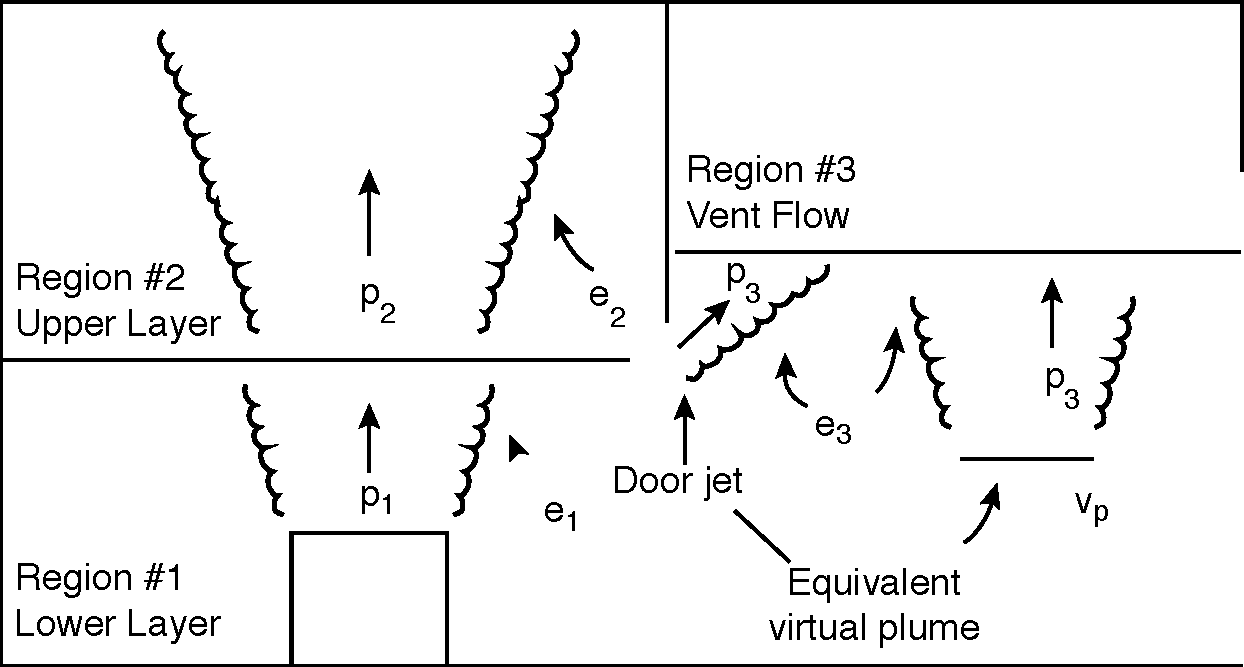
\includegraphics[width=4.0in]{FIGURES/Theory/Fire_entrain}\\
\end{center}
\caption{Entrainment and burning in a two-layer, multi-compartment model.}
 \label{fig:Burning_Regions}
\end{figure}

Initially, $\dot{m_f}$ is just the pyrolysis rate of the source fire in kg/s (region \# 1). For subsequent regions, the burning rate $\dot{m_f}$ is the unburned fuel from a previous region, $\dot{m_{tuhc}} = \dot{m_f} - \dot{m_b}$ where the subscript $tuhc$ is total unburned hydrocarbons, $f$ is the fire source, and $b$ is the amount burned.

The first step is to limit the actual burning which takes place in the combustion zone.  In each 
combustion zone, there is a quantity of fuel available.  At the source this results from the 
pyrolysis of the material, $\dot{m}_f$ .  In other situations such as a plume or door jet, it is the net 
unburned fuel available, $\dot{m}_{tuhc}$.  In each case, the fuel which is available but not burned is then 
deposited into the ``$\dot{m}_{tuhc}$ '' category.  This provides a consistent notation.  In the discussion below, 
$\dot{m}_f$  is the amount of fuel burned.  This value is initially specified as to the available fuel, and then 
reduced if there is insufficient oxygen to support complete combustion.  Subsequently, the 
available fuel, $\dot{m}_{tuhc}$, is reduced by the final value of $\dot{m}_f$ burned or $\dot{m}_b$.  Thus we have a consistent description in each burning region, with an algorithm that is invoked independent of the region being analyzed.

\be Q = \dot{m}_f H_c \ee
with the mass of oxygen required to achieve this energy release rate of
\be \dot{m}_O = \frac{Q}{E} = \dot{m}_f \frac{H_c}{E} \ee
where $E$ is the heat release per mass unit of oxygen consumed, taken to be 1.31 x $10^7$ J/kg\footnote{The units for oxygen consumption calorimetry are J/kg. The value 1.31 x $10^7$ J/kg is representative of typical fuels such as furniture (see reference \cite{Morehart:1991}) and implies these units. The variation or uncertainty (2$\sigma$) associated with this value is on the order of $\pm$ 5 \%} (based 
on oxygen consumption calorimetry for typical fuels \cite{Morehart:1991, Thornton:1917, Huggett:1980}). If the fuel contains oxygen (available for combustion), the oxygen needed to achieve full combustion is less:

\be \dot{m}_{O,needed} = \dot{m}_O - \dot{m}_{O, in the fuel} \ee

If sufficient oxygen is available, then it is fully burned.  However, if the oxygen concentration is 
low enough, it will constrain the burning and impose a limit on the amount of fuel actually 
burned, as opposed to the amount pyrolyzed.  The actual limitation is discussed below and is:

\be \dot{m}_{O.actual} = min \brackets{\dot{m}_{O,available} , \dot{m}_{O,needed}} \ee

\be \dot{m}_{f,actual} = \dot{m}_{O,actual} \frac{E}{H_c}  \ee
The relationship between oxygen and fuel concentration defines a range in which burning will 
take place.  In the CFAST model, a limit is incorporated by limiting the burning rate as the 
oxygen level decreases until a ``lower oxygen limit'' (LOL) is reached. The lower oxygen limit is 
incorporated through a smooth decrease in the burning rate near the limit:

\be \dot{m}_{O,available} = \dot{m}_eY_{O_2}C_{LOL} \ee
where $\dot{m}_e$ is the mass entrainment flow rate, $Y_{O_2}$ is the mass fraction of oxygen, and the lower oxygen limit coefficient, $C_{LOL}$  
, is the fraction of the available fuel which can be burned with the 
available oxygen and varies from 0 at the limit to 1 above the limit.  The functional form that 
utilizes the hyperbolic tangent was determined empirically to provide a smooth cutoff of the 
burning over a narrow range above the limit.

\be C_{LOL} = \frac{\tanh\brackets{{800 \brackets{Y_{O_2} - Y_{LOL}} - 400}} + 1}{2} \ee
A temperature criterion is also imposed so that no burning will take place when the temperature 
is below a user prescribed temperature.

In summary, it is possible to follow the formation of the major products of combustion (carbon 
dioxide, carbon monoxide, soot, water, hydrogen cyanide, and hydrogen chloride) using 
appropriate measured product yields (e.g., \cite{Morehart:1991}) to define product yields for eq (33). Actual 
combustion chemistry is not considered in CFAST due to the complexities associated with 
detailed kinetics and transport. 

\subsubsection{Flame Height}

CFAST includes a calculation of average flame height based on the work of Heskestad \cite{Heskestad:2002}. 
Valid for a wide range of hydrocarbon and gaseous fuels, the correlation is given by

\be H = -1.02 D + 0.235 \brackets{\frac{Q_f}{1000}} \ee
where $H$ is the average flame height, $D$ the diameter of the fire and $Q_f$ is the fire size. The mean 
flame height is defined as the distance from the fuel source to the top of the visible flame where 
the intermittency is 0.5.  A flame intermittency of 0.5 means that the visible flame is above the 
mean 50 \% of the time and below the mean 50 \% of the time.  This average flame height is 
 included in the printed output from CFAST. Note that $Q_f$ in Eq. (8) in Ref. \cite{Heskestad:2002} is in kW.
 
 \subsubsection{Limitation of the Algorithm for Fires and Mass Balance }
 
CFAST depends on pyrolysis data for the source term for a fire. The usual way to obtain this 
data is a large-scale calorimeter, e.g., reference [\cite{Bryant:2003}. Generally, a product (e.g., chair, table, 
bookcase) is placed under a large collection hood and ignited by a burner ($\approx 50$ kW simulating a wastebasket) placed adjacent to the item.  The combustion process then proceeds under assumed 
�free-burning� conditions, and the heat release rate is measured.  Potential sources of uncertainty 
include measurement errors related to the instrumentation and the degree to which �free-burn- 
ing� conditions are not achieved (e.g., radiation from the gases under the hood or from the hood 
itself, and restrictions in the air entrained by the object causing locally reduced oxygen 
concentrations affecting the combustion chemistry).  There are limited experimental data for 
upholstered furniture which suggest that prior to the onset of flashover in a compartment, the 
influence of the compartment on the burning behavior of the item is small.  The differences 
obtained from the use of different types or locations of ignition sources have not been explored. 
These factors are discussed in reference~\cite{Babrauskas:1982}. 

Where small-scale calorimeter data are used, procedures are available to extrapolate to the 
behavior of a full-size item.  These procedures are based on empirical correlations of data which 
exhibit significant scatter, thus limiting their accuracy.  For example, for upholstered furniture, 
the peak heat release rates estimated by the �triangular approximation� method averaged 91 \% 
(range 46 \% to 103 \%) of values measured for a group of 26 chairs with noncombustible frames, 
but only 63 \% (range 46 \% to 83 \%) of values measured for a group of 11 chairs with 
combustible frames \cite{Babrauskas:1985}.  Also, the triangle neglects the �tails� of the curve; these are the initial time from ignition to significant burning of the item, and the region of burning of the combusti- 
ble frame, after the fabric and filler are consumed. 

The provided data and procedures only relate directly to burning of items initiated by relatively 
large flaming sources.  Little data are currently available for release rates under smoldering 
combustion, or for the high external flux and low oxygen conditions characteristic of post- 
flashover burning.  While the model allows multiple items burning simultaneously, it does not 
account for the synergy of such multiple fires.  Thus, for other ignition scenarios, multiple items 
burning simultaneously (which exchange energy by radiation and convection), combustible 
interior finish, and post-flashover conditions, the model can give estimates which are often non- 
conservative (the actual release rates would be greater than estimated).  At present, the only sure 
way to account for all of these complex phenomena is to conduct a full-scale compartment burn 
and use the pyrolysis rates directly. 

Burning can be constrained by the available oxygen.  However, this �constrained fire� is not 
subject to the influences of radiation to enhance its burning rate, but is influenced by the oxygen 
available in the compartment.  If a large mass loss rate is entered, the model will follow this 
input until there is insufficient oxygen available for that quantity of fuel to burn in the 
compartment.  The unburned fuel (sometimes called excess pyrolysate) is tracked as it flows out 
in the door jet, where it can entrain more oxygen.  If this mixture is within the user-constrained 
flammable range, it burns in the door plume.  If not, it will be tracked throughout the building 
until it eventually collects as unburned fuel or burns in a vent.  The enthalpy released in the fire 
compartment and in each vent, as well as the total enthalpy released, is detailed in the output of 
the model.  Since mass and enthalpy are conserved, the total will be correct.  However, since 
combustion did not take place adjacent to the burning object, the actual mass burned could be 
lower than that specified by the user.  The difference will be the unburned fuel. 

An oxygen combustion chemistry scheme is employed only in constrained fires.  Here user- 
constrained hydrocarbon ratios and species yields are used by the model to predict concentra- 
tions.  A balance among hydrogen, carbon, and oxygen molecules is maintained.  Under some 
conditions, low oxygen can change the combustion chemistry, with a resulting increase in the 
yields of products of incomplete combustion such as carbon monoxide. However, not enough is 
known about these chemical processes to build this relationship into the model at the present 
time.  Some data exist in reports of full-scale experiments (e.g., reference \cite{Lee:1982}) which can assist in making such determinations.

\subsection{Plumes} 

A plume is formed above any burning object.  It acts as a pump transferring mass and enthalpy 
from the lower layer into the upper layer.  A correlation is used to predict the amount of mass 
and enthalpy that is transferred.  A more complete plume model would predict plume 
entrainment by creating a separate zone and solving the appropriate equations.

Two sources exist for moving enthalpy and mass between the layers within and between 
compartments.  Within the compartment, the fire plume provides one source.  The other source 
of mixing between the layers occurs at vents such as doors or windows.  Here, there is mixing at 
the boundary of the opposing flows moving into and out of the compartment.  The degree of 
mixing is based on an empirically-derived mixing relation.  Both the outflow and inflow entrain 
air from the surrounding layers.  The flow at vents is also modeled as a plume (called the door 
plume or jet), and uses the same equations as the fire plume, with two differences.  First, an 
offset is calculated to account for entrainment within the doorway and second, the equations are 
modified to account for the rectangular geometry of vents compared to the round geometry of 
fire plumes.  All plumes within the simulation entrain air from their surroundings according to 
an empirically-derived entrainment relation.  Entrainment of relatively cool, non-smoke laden air 
adds oxygen to the plume and allows burning of the fuel.  It also causes it to expand as the plume 
moves upward in the shape of an inverted cone.  The entrainment in a vent is caused by bi- 
directional flow and results from vortices formed near a shear layer.  This phenomenon is called 
the Kelvin-Helmholtz instability \cite{Alterman:1961}.  It is not exactly the same as a normal plume, so some error (not measured) arises when this entrainment is approximated by a normal plume 
entrainment algorithm. 

While experiments show that there is very little mixing between the layers at their interface, 
sources of convection such as radiators or diffusers of heating and air conditioning systems, and 
the downward flows of gases caused by cooling at walls, will cause such mixing.  These are 
examples of phenomena which are inconsistent with the two-zone approximation.  Also, the 
plumes are assumed not to be affected by other flows which may occur.  For example, if the 
burning object is near the door the strong inflow of air will cause the plume axis to lean away 
from the door and affect entrainment of gases into the plume.  Such effects are not included in 
the model. 

As discussed above, each compartment is divided into an upper and lower layer.  At the start of 
the simulation, the layers in each compartment are initialized at ambient conditions and by 
default, the upper layer volume set to 0.001 of the compartment volume (an arbitrary, small 
value set to avoid the potential mathematical problems associated with dividing by zero).  Other 
values can be set.  As enthalpy and mass are pumped into the upper layer by the fire plume, the 
upper layer expands in volume causing the lower layer to decrease in volume and the interface to 
move downward.  If the door to the next compartment has a soffit, there can be no flow through 
the vent from the upper layer until the interface reaches the bottom of that soffit.  Thus in the 
early stages the expanding upper layer will push down on the lower layer air and force it into the 
next compartment through the vent by expansion.  

Once the interface reaches the soffit level, a door plume forms and flow from the fire connecting doorway compartment to the next compartment is initiated.  As smoke flow from the fire compartment 
fills the second compartment, the lower layer of air in the second compartment is pushed down. 
As a result, some of this air flows into the fire compartment through the lower part of the (or vent).  Thus, a vent between the fire compartment and connecting compartments can have simultaneous, opposing flows of air.  All flows are driven by pressure and density differences that result from temperature differences and layer depths. The key to getting the correct flow is to distribute correctly the fire and plume�s mass and enthalpy between the layers. 

Buoyancy generated by the combustion processes in a fire causes the formation of a plume. 
Such a plume can transport mass and enthalpy from the fire into the lower or upper layer of a 
compartment.  In the present implementation, we assume that both mass and enthalpy from the 
fire are deposited only into the upper layer.  In addition the plume entrains mass from the lower 
layer and transports it into the upper layer.  This yields a net enthalpy transfer between the two 
layers. 

A fire generates energy at a rate $Q_f$.  Some fraction, $\chi_R$, will exit the fire as radiation.  The 
remainder, $\chi_C$, will then be deposited in the layers as convective energy or heat additional fuel 
which may then pyrolyze. McCaffrey \cite{McCaffrey:1983} estimated the mass entrained by the fire/plume from the lower into the upper layer. This correlation divides the flame/plume into three regions as 
given in eq \ref{eq:McCaffreyPlume}.  This prescription agrees with the work of Cetegen et al. \cite{Cetegen:1982, Cetegen:1984} in the intermittent regions but yields greater entrainment in the other two regions.  This difference is particularly important for the initial fire since the upper layer is far removed from the fire.

\begin{eqnarray}
\textnormal{flaming:} & \frac{\dot{m}_e}{Q_f} = 0.011 \brackets{\ZQf}^{0.566} & 0.00 \leq \brackets{\ZQf}<0.08 \nonumber \\
\textnormal{intermittent:} & \frac{\dot{m}_e}{Q_f} = 0.026 \brackets{\ZQf}^{0.909} & 0.08 \leq \brackets{\ZQf}<0.20 \label{eq:McCaffreyPlume} \\
\textnormal{plume} & \frac{\dot{m}_e}{Q_f} = 0.124 \brackets{\ZQf}^{1.895} & 0.20 \leq \brackets{\ZQf} \nonumber
\end{eqnarray}
McCaffrey's correlation is an extension of the common point source plume model, with a 
different set of coefficients for each region. These coefficients are experimental correlations. 

Within CFAST, the radiative fraction defaults to 0.30 \cite{Drysdale:1985}; i.e., 30 \% of the fire�s energy is released via radiation.  For other fuels, the work of Tewarson \cite{Tewarson:1978}, McCaffrey \cite{McCaffrey:1982}, or Koseki \cite{Koseki:1989} is available for reference.  The typical range for the radiative fraction is from about 0.05 to 0.4.
 
In CFAST, there is a constraint on the quantity of gas which can be entrained by a plume arising 
from a fire.  The constraint arises from the physical fact that a plume can rise only so high for a given size of a heat source.  Early in a fire, when the energy flux is very small, the plume may 
not have sufficient energy to reach the compartment ceiling. The correct sequence of events is 
for a small fire to generate a plume which does not reach the ceiling or upper layer initially.  The 
plume entrains enough cool gas to decrease the buoyancy to the point where it no longer rises. 
When there is sufficient energy present in the plume, it will penetrate the upper layer.  To this 
end the following prescription has been incorporated:  for a given size fire, a limit is placed on 
the amount of mass which can be entrained, such that no more is entrained than would allow the 
plume to reach the layer interface.  The result is that the interface falls at about the correct rate, 
although it starts a little too soon, and the upper layer temperature is over predicted, but follows 
experimental data after the initial phase. 

For the plume to be able to penetrate the inversion formed by a hot gas layer over a cooler gas 
layer, the density of the gas in the plume at the point of intersection must be less than the density 
of the gas in the upper layer. In practice, this places a maximum on the air entrained into the 
plume. From conservation of mass and enthalpy

\be \dm_p = \dm_f + \dm_e \label{eq:plume_mass} \ee

\be \dm_pc_pT_p = \dm_fc_pT_f + \dm_ec_pT_l \label{eq:plume_energy} \ee
where the subscripts $p$, $f$, $e$, and $l$ refer to the plume, fire, entrained air, and lower layer, 
respectively.

The criterion that the density in the plume region be lower than the upper layer implies that $T_u~<~T_p$. Solving eq \ref{eq:plume_energy} for $T_p$ and substituting for $\dm_p$ from \ref{eq:plume_mass} yields

\be T_p = \frac{T_f\dm_f + T_l\dm_e}{\dm_f + \dm_e} > T_u \ee
or
\be \dm_e < \brackets{\frac{T_f - T_u}{T_u - T_l}}\dm_f < \frac{T_f}{T_u - T_l} \dm_f \label{eq:entrainment_limit} \ee
 Substituting the convective energy released by the fire, $Q_{f,c} = \dm_fc_pT_f$, into eq \ref {eq:entrainment_limit} yields the form of the  entrainment limit use in the CFAST model:
 
 \be \dm_e < \frac{Q_{f,c}}{c_p\brackets{T_u - T_l}} \ee
 which is incorporated into the model.  It should be noted that both the plume and layers are 
assumed to be well mixed with negligible mixing and transport time for the plume and layers. 

\subsubsection{Limitation of the Plume Algorithm }

The entrainment coefficients are empirically determined values from the work of McCaffrey \cite{McCaffrey:1983}. Small errors in these values will have a small effect on the fire plume or the flow in the plume of gases exiting the door of that compartment.  In a multi-compartment model such as 
CFAST, however, small errors in each door plume are multiplicative as the flow proceeds 
through many compartments, possibly resulting in a significant error in the furthest 
compartments.  The data available from validation experiments \cite{Peacock:1988} discussed in the CFAST Validation Guide \cite{CFAST_Valid_Guide_6} indicate that the values for entrainment coefficients currently used in most zone models produce good agreement for a 
three-compartment configuration.  More data are needed for larger numbers of compartments to 
study this further. 

In real fires, smoke and gases are introduced into the lower layer of each compartment primarily 
due to mixing at connections between compartments and from the downward flows along walls 
(where contact with the wall cools the gas and reduces its buoyancy).  Doorway mixing has been 
included in CFAST, using the same empirically derived mixing coefficients as used for 
calculating fire plume entrainment. Downward wall flow has not been included. This could 
result in underestimates of lower layer temperatures and species concentration. 
Entrainment at a vent (doors, windows, ...) yields mixing into the lower and upper layers. The 
latter has been studied more extensively than the former. The door jets are not symmetric for 
these mixing phenomena, however.  We have constrained the phenomenon for CFAST to be in 
the range as predicted by Zukoski et al. \cite{Zukoski:1985}. 

\subsection{Vent Flow}

Flow through vents is a dominant component of any fire model because it is sensitive to small changes in pressure and transfers the greatest amount of enthalpy on an instantaneous basis of all the source terms (except of course for the fire and plume).  Its sensitivity to environmental changes arises through its dependence on the pressure difference between compartments which can change rapidly.  

CFAST models two types of vent flow, vertical flow through horizontal vents (such as ceiling holes or hatches) and horizontal flow through vertical vents (such as doors or windows).  Horizontal flow is the flow which is normally thought of when discussing fires.  Vertical flow is particularly important in two disparate situations: a ship, and the role of fire fighters doing roof venting.

Horizontal vent flow is determined using the pressure difference across a vent.  Flow at a given elevation may be computed using Bernoulli�s law by first computing the pressure difference at that elevation.  The pressure on each side of the vent is computed using the pressure at the floor, the height of the floor and the density. 

Atmospheric pressure is about 100~000 Pa. Fires produce pressure changes from 1~Pa to 1~000~Pa and mechanical ventilation systems typically involve pressure differentials of about 1~Pa to 100~Pa.  The pressure variables are solved to a higher accuracy than other solution variables because of the subtraction (with resulting loss of precision) needed to calculate vent flows from pressure differences.

Mass flow (in the remainder of this section, the term ``flow'' will be used to mean mass flow) is the dominant source term for the predictive equations because it fluctuates most rapidly and transfers the greatest amount of enthalpy on an instantaneous basis of all the source terms (except of course the fire).  Also, it is most sensitive to changes in the environment.  Horizontal flow encompasses flow through doors, windows and so on. Horizontal flow is discussed in section 3.4.3.1. Vertical flow occurs in ceiling vents.  It is important in two separate situations: on a ship with open hatches and in house fires with roof venting.  Vertical flow is discussed in section 3.4.3.2.

Flow through vents can be forced (mechanical) or natural (convective). Force flow can occur through either vertical or horizontal vents. The differences are primarily the selection rules for the source of the gases or whether the resultant plume enters the lower or upper layer of each compartment.

There is a special case of horizontal flow for long corridors. A corridor flow algorithm is incorporated to calculate the time delay from when a plume enters a compartment to when the effluent is available for flow into adjacent compartments.

Flow through vents can be modified, that is turned on or off. This applies to the three types of vents discussed below, horizontal flow through vertical vents (HVENT), vertical flow through horizontal vents (VVENT) and forced flow (MVENT). For each key word, there is a an initial opening fraction which is reflected in the first region in figure \ref{fig:Opening_Fraction}. This initial opening fraction can be modified by by the EVENT key word to change the fraction. This change occurs over a transition time which defaults to one second. The final fraction is the third region depicted in figure \ref{fig:Opening_Fraction}. There can be only a single transition per vent.

\begin{figure}[t]
\begin{center}
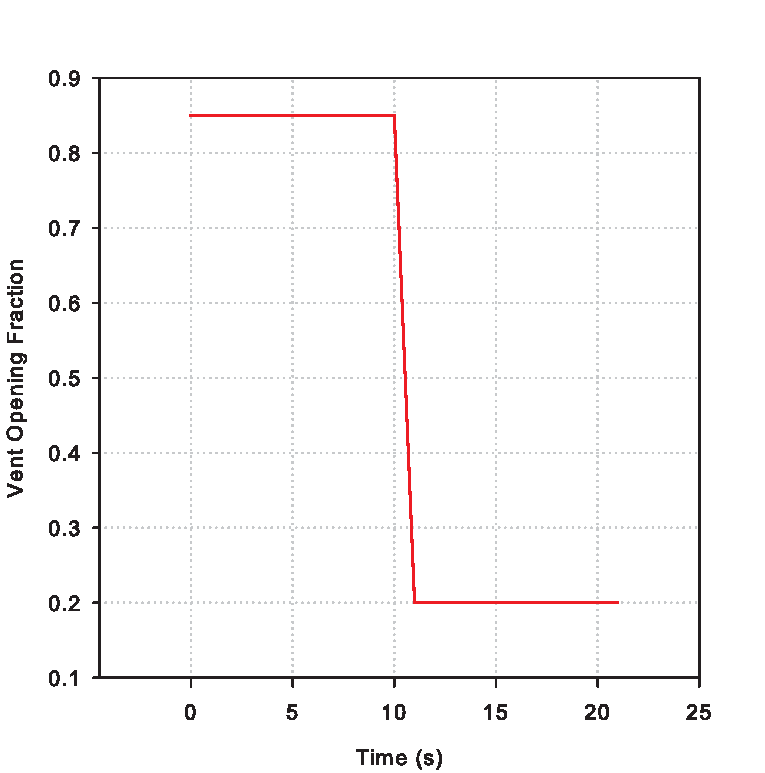
\includegraphics[width=4.0in]{FIGURES/Theory/Opening_Fraction}\\
\end{center}
\caption{Vent opening size fraction as a function of time.}
 \label{fig:Opening_Fraction}
\end{figure}

\subsubsection{Horizontal Flow Through Vertical Vents}

Flow through normal vents such as windows and doors is governed by the pressure difference across a vent.  A momentum equation for the zone boundaries is not solved directly.  Instead momentum transfer at the zone boundaries is included by using an integrated form of Euler's equation, namely Bernoulli's solution for the velocity equation.  This solution is augmented for restricted openings by using flow coefficients \cite{Quintiere:1984} to allow for constriction from finite size doors.  The flow (or orifice) coefficient is an empirical term which addresses the problem of constriction of velocity streamlines at an orifice.

Bernoulli's equation is the integral of the Euler equation and applies to general initial and final velocities and pressures.  The implication of using this equation for a zone model is that the initial velocity in the doorway is the quantity sought, and the final velocity in the target compartment vanishes.  That is, the flow velocity vanishes where the final pressure is measured.  Thus, the pressure at a stagnation point is used.  This is consistent with the concept of uniform zones which are completely mixed and have no internal flow.  The general form for the velocity of the mass flow is given by

\be v = C \sqrt{\frac{2 \Delta P}{\rho}} \ee


where $C$ is the constriction (or flow) coefficient (�0.7), $\rho$ is the gas density on the source side, and $\Delta P$ is the pressure across the interface.  (Note: at present we use a constant value for $C$ for all gas temperatures).

The simplest means to define the limits of integration is with neutral planes, that is the height at which flow reversal occurs, and physical boundaries such as sills and soffits.  By breaking the integral into intervals defined by flow reversal, a soffit, a sill, or a zone interface, the flow equation can be integrated piecewise analytically and then summed.  

The approach to calculating the flow field is of some interest.  The flow calculations are performed as follows.  The vent opening is partitioned into at most six slabs where each slab is bounded by a layer height, neutral plane, or vent boundary such as a soffit or sill.  The most general case is illustrated in figure \ref{Fig:Flow_Notation}.

\begin{figure}[t]
\begin{center}
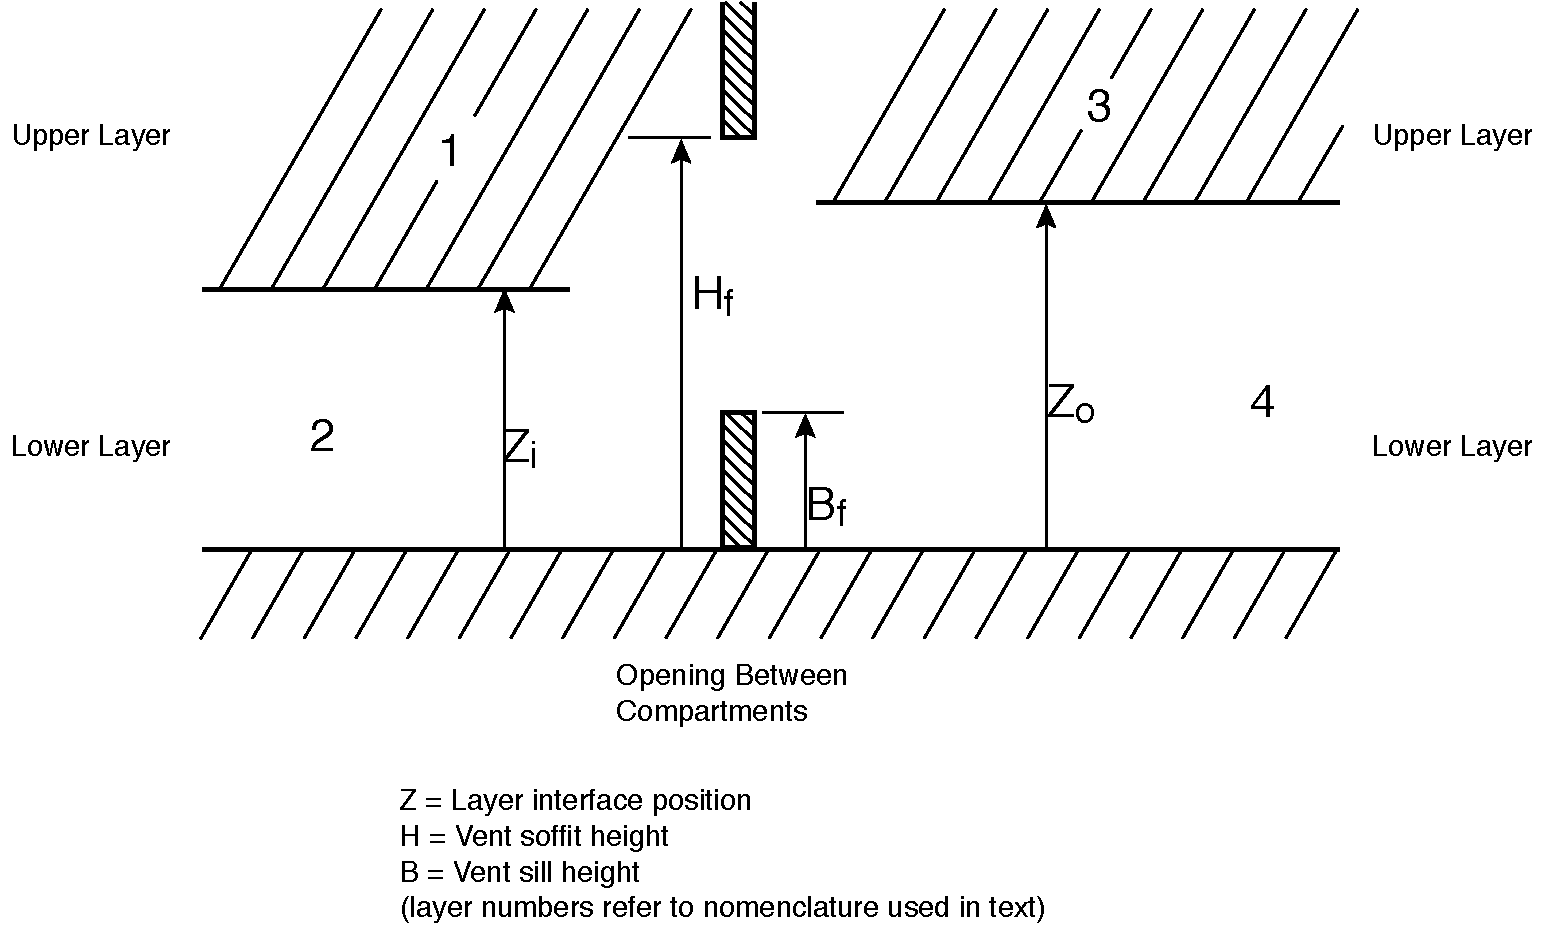
\includegraphics[width=5.0in]{FIGURES/Theory/Flow_Notation}\\
\end{center}
\caption{Vent opening size fraction as a function of time.}
 \label{fig:Flow_Notation}
\end{figure}

The mass flow for each slab can be determined from

\be \dm_{io} = \frac{1}{3} C \brackets{8 \rho} A_{slab} \brackets{\frac{x^2+xy+y2}{x+y}} \ee
where $x = \sqrt{|P_t|}$ and $y = \sqrt{|P_b|}$. $P_t$ and $P_b$ are the cross-vent pressure differential at the top and bottom of the slab respectively and $A_{slab}$ is the cross-sectional area of the slab.  The value of the density, $\rho$, is taken from the source compartment.

A mixing phenomenon occurs at vents which is similar to entrainment in plumes.  As hot gases from one compartment leave that compartment and flow into an adjacent compartment a door jet can exist which is analogous to a normal plume.  Mixing of this type occurs for $\dm_{13} > 0$ as shown in figure \ref{fig:Flow_Patterns}.  To calculate the entrainment ($\dm_{43}$ in this example), once again we use a plume description consistent with the work of McCaffrey, but with an extended point source.  The estimate for the point source extension is given by Cetegen et al. \cite{Cetegen:1984}.  This virtual point source is chosen so that the flow at the door opening would correspond to a plume with the heating for a equivalent doorway fire source (with respect to the lower layer) given by

\begin{figure}[t]
\begin{center}
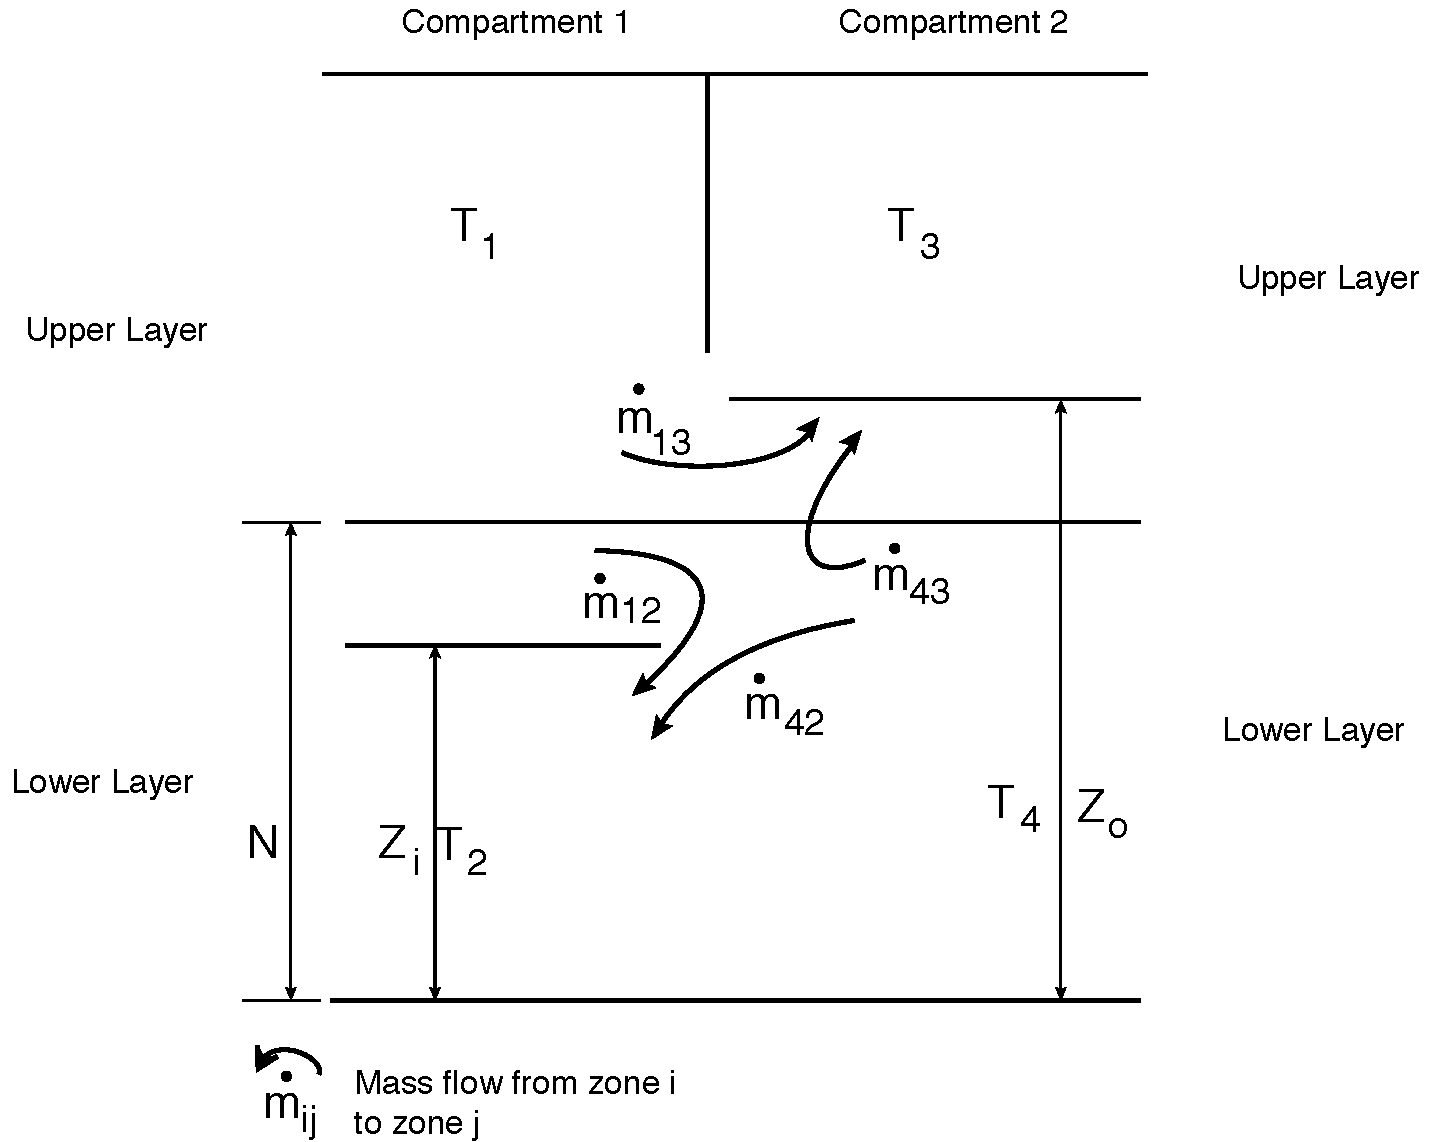
\includegraphics[width=5.0in]{FIGURES/Theory/Flow_Patterns}\\
\end{center}
\caption{Flow patterns and layer number conventions for horizontal flow through a vertical vent.}
 \label{fig:Flow_Patterns}
\end{figure}

\be Q_{f,eq} = c_p \brackets{T_l-T_4} \dm_{13} \ee
where $Q_{f,eq}$ is the heat release rate of the doorway fire. The concept of the virtual source is that the enthalpy flux from the virtual point source should equal the actual enthalpy flux in the door jet at the point of exit from the vent using the same prescription.  Thus the entrainment is calculated the same way as was done for a normal plume.  The reduced height of the plume, $z_p$, is

\be z_p = \frac{z_13}{Q_{f,eq}^{2/5}}+ v_p \ee
where $v_p$ the virtual point source, is defined by inverting the entrainment process to yield

\begin{eqnarray} 
v_P = \brackets{\frac{90.9 \dm}{Q_{f,eq}}}^{1.76} & 0.00 < v_p \leq 0.08 \nonumber \\
v_P = \brackets{\frac{38.5 \dm}{Q_{f,eq}}}^{1.001} & 0.08 < v_p \leq 0.20 \label{eq:McCaffreyPlume} \\
v_P = \brackets{\frac{8.10 \dm}{Q_{f,eq}}}^{0.528} & 0.20 < v_p \nonumber \nopagebreak
\end{eqnarray}

Although outside of the normal range of validity of the plume model, a level of agreement with experiment is apparent (section 6 includes discussion of validation experiments for the plume model).  Since a door jet forms a flat plume whereas a normal fire plume will be approximately circular, strong agreement is not expected.

The other type of mixing is much like an inverse plume and causes contamination of the lower layer.  It occurs when there is flow of the type $\dm_{42} > 0$.  The shear flow causes vortex shedding into the lower layer and thus some of the particulates end up in the lower layer.  The actual amount of mass or energy transferred is usually not large, but its effect can be large.  For example, even minute amounts of carbon can change the radiative properties of the gas layer, from negligible to something finite.  It changes the rate of radiation absorption significantly and invalidates the simplification of an ambient temperature lower layer.  This term is predicated on the Kelvin-Helmholz flow instability and requires shear flow between two separate fluids.  The mixing is enhanced for greater density differences between the two layers. However, the amount of mixing has never been well characterized. Quintiere et al. \cite{Quintiere:1984} discuss this phenomena for the case of crib fires in a single room, but their correlation does not yield good agreement with experimental data in the general case \cite{Quintiere:1981}.  In the CFAST model, it is assumed that the incoming cold plume behaves like the inverse of the usual door jet between adjacent hot layers; thus we have a descending plume. It is possible that the entrainment is overestimated in this case, since buoyancy, which is the driving force, is not nearly as strong as for the usually upright plume.

\subsubsection{Vertical Flow Through Horizontal Vents}

Flow through a ceiling or floor vent can be somewhat more complicated than through door or window vents.  The simplest form is uni-directional flow, driven solely by a pressure difference.  This is analogous to flow in the horizontal direction driven by a piston effect of expanding gases.  Once again, it can be calculated based on the Bernoulli equation, and presents little difficulty.  However, in general we must deal with more complex situations that must be modeled in order to have a proper understanding of smoke movement.  The first is an occurrence of puffing.  When a fire exists in a compartment in which there is only one hole in the ceiling, the fire will burn until the oxygen has been depleted, pushing gas out the hole.  Eventually the fire will die down.  At this point ambient air will rush back in, enable combustion to increase, and the process will be repeated.  Combustion is thus tightly coupled to the flow.  The other case is exchange flow which occurs when the fluid configuration across the vent is unstable (such as a hotter gas layer underneath a cooler gas layer).  Both of these pressure regimes require a calculation of the onset of the flow reversal mechanism.

Normally a non-zero cross vent pressure difference tends to drive unidirectional flow from the higher to the lower pressure side.  An unstable fluid density configuration occurs when the pressure alone would dictate stable stratification, but the fluid densities are reversed.  That is, the hotter gas is underneath the cooler gas.  Flow induced by such an unstable fluid density configuration tends to lead to bi-directional flow, with the fluid in the lower compartment rising into the upper compartment.  This situation might arise in a real fire if the room of origin suddenly had a hole punched in the ceiling. No pretense is made of being able to do this instability calculation analytically. Cooper's algorithm \cite{Cooper:1989} is used for computing mass flow through ceiling and floor vents. It is based on correlations to model the unsteady component of the flow.  What is surprising is that we can find a correlation at all for such a complex phenomenon. There are two components to the flow.  The first is a net flow dictated by a pressure difference. The second is an exchange flow based on the relative densities of the gases.  The overall flow is given by \cite{Cooper:1989, Cooper:1990, Cooper:1995}

\be \dm = C f\brackets{\gamma, \epsilon} \sqrt{\frac{\Delta P}{\overline{\rho}}} A_v \ee
where $\gamma = c_p/c_v$ is the ratio of specific heats, $C = 0.68 + 0.17 \epsilon$, $\epsilon = \frac{\Delta P}{P}$, and $f$ us a weak function of both $\gamma$ and $\epsilon$ \cite{Cooper:1989}. In the situation where we have an instability, we use Cooper's correlations for the function $f$.  The resulting exchange flow is given by

\be \dm_{ex} = 0.1 \brackets{\frac{g \Delta \rho A_v^{5/2}}{\rho_{av}}} \brackets{1.0 - \frac{2 A_v^2 \Delta P}{S^2 g \Delta \rho D^5}} \ee
where $D = 2 \sqrt{A_v / \pi}$ and $S$ is 0.754 for round or 0.942 for square openings, respectively \cite{Cooper:1989}. Vertical flow through horizontal vents is governed by the VFLOW routines. VENTCF is the module which calculates the mass flow from one compartment to another. The values returned are $\dm_{incoming}$ and $\dm_{outgoing}$ through each vent. These terms are symmetric: the outgoing flow from compartment 1 to 2 is the same as incoming flow from compartment 2 to 1, though source and destination layers may be different. 

The energy flux into a compartment is then determined by the relative size and temperature of the layers of the compartment from which the mass is flowing (incoming, u and l):

\be \dq_{incoming} = c_p \dm_u T_u + c_p \dm_l T_l \ee

\be \dm_u = \dm_{incoming} \frac{V_u}{V} \ee

\be \dm_l = \dm_{incoming} \frac{V_l}{V} \ee


The mass and energy are then deposited into the upper or lower layer of the receiving compartment based on the effective temperature of the incoming flow relative to the upper and lower layers of the receiving compartment. If the temperature of the incoming flow is higher than the temperature of the lower layer, then the flow is deposited into the upper layer. This is similar to the usual plume from a fire or a doorway jet. These rules are implemented in VFLOW.

\subsubsection{Forced Flow}

Forced flow in this version of CFAST is a supply (or exhaust) system based on constant flow through a opening/fan/opening triplet . These systems are commonly used in buildings for heating, ventilation, air conditioning, pressurization, and exhaust. Figure \ref{fig:Fans_and_Ducts}(a) shows smoke management by an exhaust fan at the top of an atrium, and figure \ref{fig:Fans_and_Ducts}(b) illustrates a kitchen exhaust.  Cross ventilation, shown in figure \ref{fig:Fans_and_Ducts}(c), is occasionally used without heating or cooling.  Generally systems that maintain comfort conditions have either one or two fans.

\begin{figure}
\begin{center}
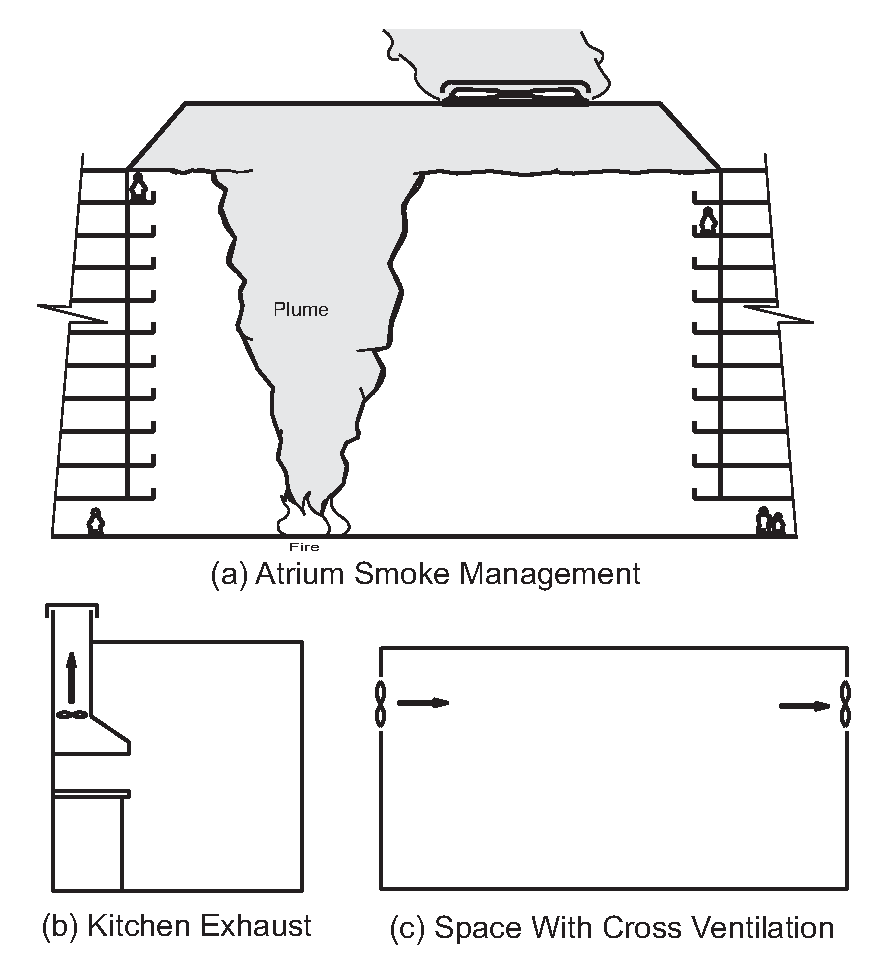
\includegraphics[width=5.0in]{FIGURES/Theory/HVAC_Fans_and_Ducts}\\
\end{center}
\caption{Some simple fan-duct systems.}
 \label{fig:Fans_and_Ducts}
\end{figure}

Further information about these systems is presented in Klote and Milke \cite{Klote:2002} and the American Society of Heating, Refrigerating and Air Conditioning Engineers (ASHRAE) \cite{ASHRAE:2001}.

This version of the model does not include duct work or variable fans. These equations are high-order, non-linear and in some cases ill-posed, which caused a great deal of difficulty in reaching a numerical solution.

The flow through mechanical vents can be filtered. Filtering affects particulates such as smoke and the trace species. Filtering can be turned on at any time. Effectiveness is from 0~\% (no effect) to 100~\% which completely blocks flow of these two species.

\subsubsection{Corridor Flow}

A standard assumption in zone fire modeling is that once hot smoke enters a compartment, a well defined upper layer forms instantly throughout the compartment. This assumption breaks down in large compartments and long corridors due to the time required to fill these spaces.  A simple procedure is described for accounting for the formation delay of an upper layer in a long corridor by using correlations developed from numerical experiments generated with the NIST fire model Large Eddy Simulation Model (LES) , which is now the Fire Dynamic Simulation Model (FDS) \cite{FDS_Tech_Guide_5}.  FDS is a computational fluid dynamics model capable of simulating fire flow velocities and temperatures with high ($\approx$0.1 m) resolution.  Two parameters related to corridor flow are then estimated: the time required for a ceiling jet to travel in a corridor and the temperature distribution down the corridor.  These estimates are then used in CFAST by delaying flow into compartments connected to corridors until the ceiling jet has passed these compartments.

FDS was used to estimate ceiling jet characteristics by running a number of cases for various inlet layer depths and temperatures. The vent flow algorithm in CFAST then uses this information to compute mass and enthalpy flow between the corridor and adjacent compartments. This is accomplished by presenting the vent algorithm with a one layer environment (the lower layer) before the ceiling jet reaches the vent and a two layer environment afterwards. Estimated ceiling jet temperatures and depths are used to define upper layer properties.

The problem is to estimate the ceiling jet temperature and depth as a function of time until it reaches the end of the corridor.  The approach used here is to run a field model as a pre-processing step and to summarize the results as correlations describing the ceiling jet's temperatures and velocities. The steps used in this process are as follows:

\begin{enumerate}
\item Model corridor flow for a range of inlet ceiling jet temperatures and depths. Inlet velocities are derived from the inlet temperatures and depths.

\item For each model run calculate average ceiling jet temperature and velocity as a function of distance down the corridor.

\item Correlate the temperature and velocity distribution down the hall.
\end{enumerate}


The zone fire model then uses these correlations to estimate conditions in the corridor as follows:

\begin{enumerate}
\item Estimate the inlet temperature, depth and velocity of the ceiling jet. If the corridor is the fire room then use a standard correlation.  If the source of the ceiling jet is another room then calculate the inlet ceiling jet flow using Bernoulli's law for the vent connecting the source room and the corridor.

\item Use correlations in 3. above to estimate the ceiling jet arrival time at each vent.

\item For each vent in the corridor use lower layer properties to compute vent flow before the ceiling jet arrives at the vent and lower/upper layer properties afterwards.
\end{enumerate}


{\bf Assumptions:} The assumptions made in order to develop the correlations are:

\begin{itemize}
\item The time scale of interest is the time required for a ceiling jet to traverse the length of the corridor. For example, for a 100~m corridor with 1 m/s flow, the characteristic time would be 100~s.

\item Cooling of the ceiling jet due to mixing with adjacent cool air is large compared to cooling due to heat loss to walls. Equivalently, we assume that walls are adiabatic.  This assumption is conservative. An adiabatic corridor model predicts more severe conditions downstream in a corridor than a model that accounts for heat transfer to walls, since cooler ceiling jets travel slower and not as far.

\item We do not account for the fact that ceiling jets that are sufficiently cooled will stagnate. Similar to the previous assumption, this assumption is conservative and results in over predictions of conditions in compartments connected to corridors (since the model predicts that a ceiling jet may arrive at a compartment when in fact it may have stagnated before reaching it).

\item Ceiling jet flow is buoyancy driven and behaves like a gravity current.  The inlet velocity of the ceiling jet is related to its temperature and depth.

\item Ceiling jet flow lost to compartments adjacent to the corridor is not considered when estimating ceiling jet temperatures and depths. Similarly, a ceiling jet in a corridor is assumed to have only one source.

\item The temperature and velocity at the corridor inlet is constant in time.

\item The corridor height and width do not effect a ceiling jet's characteristics. Two ceiling jets with the same inlet temperature, depth and velocity behave the same when flowing in corridors with different widths or heights as long as the ratio of inlet widths to corridor width are equal.

\item Flow entering the corridor enters at or near the ceiling. The inlet ceiling jet velocity is reduced from the vent inlet velocity by a factor of wvent/wroom where wvent and wroom  are the width of the vent and room, respectively.
\end{itemize}

{\bf Corridor Jet Flow Characteristics:} Ceiling jet flow in a corridor can be characterized as a one dimensional gravity current. To a first approximation, the velocity of the current depends on the difference between the density of the gas located at the leading edge of the current and the gas in the adjacent ambient air.  The velocity also depends on the depth of the current below the ceiling. A simple formula for the gravity current velocity may be derived by equating the potential energy of the current, $mgd_0/2$, measured at the half-height $d_0/2$ with its kinetic energy, $mV^2/2$ to obtain

\be V = \sqrt{g d_0} \ee
where $m$ is mass, $g$ is the acceleration of gravity, $d_0$ is the height of the gravity current and $V$ is the velocity. When the density difference, between the current and the ambient fluid is small, the velocity, $V$, is proportional to $\sqrt{g d_0 \Delta \rho / \rho_{cj}}$ = $\sqrt{g d_0 \Delta T / T_{amb}}$ where $\rho_{amb}$ and $T_{amb}$ are the ambient density and temperature and $\rho_{cj}$ and $T_{cj}$ are the density and temperature of the ceiling jet and  $\Delta T = T_{cj} - T_{amb}$ is the temperature difference. Here use has been made of the ideal gas law, $\rho_{amb} T_{amb} \approx \rho_{cj} T_{cj}$.  This can be shown using an integrated form of Bernoulli's law noting that the pressure drop at the bottom of the ceiling jet is $P_b = 0$, the pressure drop at the top is $P_t = gd_0(\rho_{cj} - \rho_{amb})$ and using a vent coefficient cvent of 0.74, to obtain

\begin{eqnarray} 
V_0 & = & c_{vent} \frac{\sqrt{8}}{3} \frac{1}{\sqrt{\rho_{cj}}} \frac{P_t + \sqrt{P_tP_b}+P_b}{\sqrt{P_t} + \sqrt{P_b}} \nonumber \\
 & = & c_{vent} \frac{\sqrt{8}}{3} \sqrt{\frac{P_t}{\rho_{cj}}} \nonumber \\
 & = & c_{vent} \frac{\sqrt{8}}{3} \sqrt{g d_0 \frac{\rho_{amb} - \rho_{cj}}{\rho_{cj}}} \nonumber \\
 & \approx & 0.7 \sqrt{g d_0 \frac{\Delta T}{T_{amb}}} \label{eq:Corridor_Flow}
 \end{eqnarray}
 
Formulas of the form of the above equation lead one to conclude that a ceiling jet's characteristics in a corridor depend on its depth, $d_0$, and relative temperature difference, $\Delta T/T_{amb}$. Therefore, as the jet cools, it slows down. If no heat transfer occurs between the ceiling jet and the surrounding walls, then the only mechanism for cooling is mixing with surrounding cool air.

Twenty numerical experiments were performed using FDS in order to better understand the effects of the inlet ceiling jet temperature and depth on ceiling jet characteristics downstream in a corridor.  These cases were run with five different inlet depths and four different inlet temperatures.  The inlet ceiling jet temperature rise, $\Delta T_0$, and depth, $d_0$, were used to define an inlet velocity, $V_0$ using eq (\ref{eq:Corridor_Flow}).  The inlet ceiling jet depths, $d_0$, used in the parameter study are 0.15 m, 0.30 m, 0.45 m, 0.60 m and 0.75 m. The inlet ceiling jet temperature rises, $T_0$, used in the parameter study are 100 \degc, 200 \degc, 300 \degc and 400 \degc.

{\bf Correlations:} Ceiling jet functions were plotted as a function of distance down a corridor for each of the 20 test cases.  These results are shown in figure \ref{fig:Corr_Flow}.  Note that all but the 0.15 m ceiling jet data lie on essentially the same line. 

\begin{figure}
\begin{center}
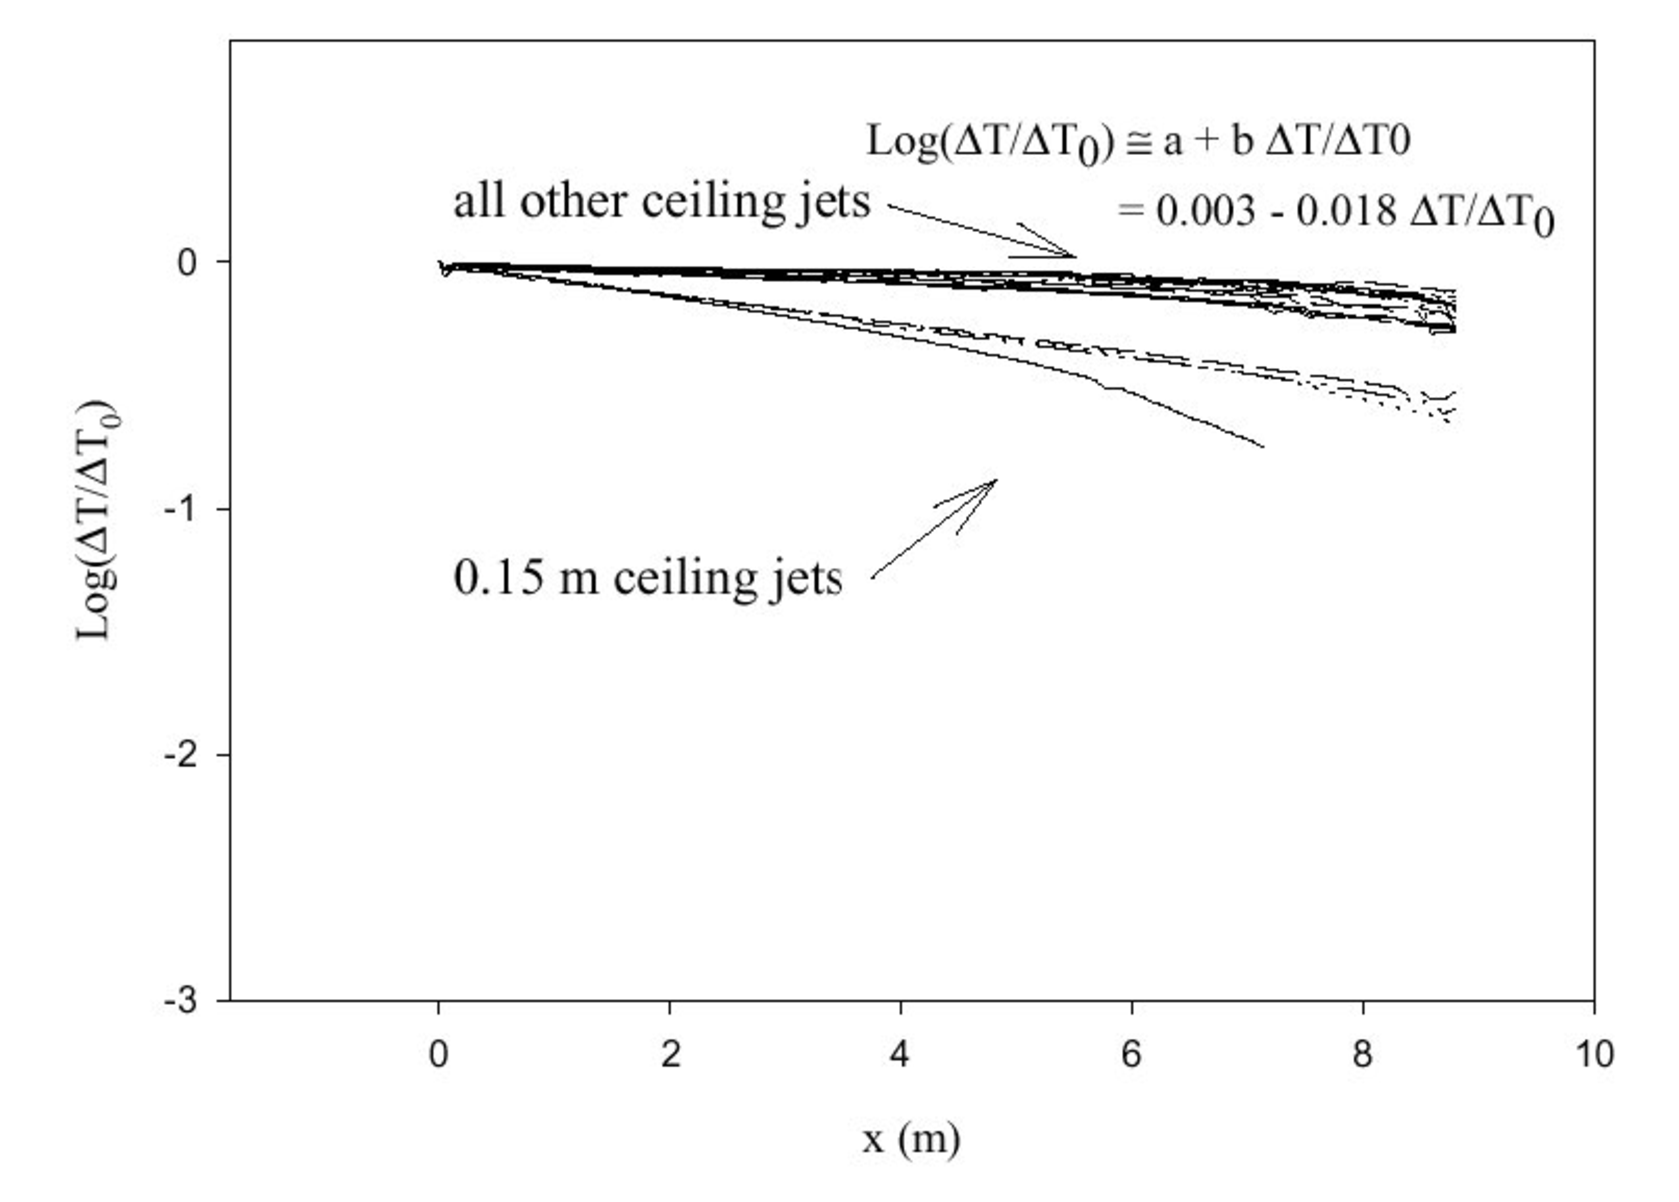
\includegraphics[width=5.0in]{FIGURES/Theory/Corr_Flow}\\
\end{center}
\caption{Relative excess downstream temperature in a corridor using an adiabatic temperature boundary condition for several inlet depths and inlet temperature boundary conditions. The inlet velocity is given by eq (\ref{eq:Corridor_Flow}).}
 \label{fig:Corr_Flow}
\end{figure}

The best fit line is given in the form of $\log{\frac{\Delta T}{\Delta T_0}} = a + bx$. This is equivalent to 

\be \frac{\Delta T}{\Delta T_0} = C_1 10^{bx}  = C_1 \brackets{\frac{1}{2}}^{x/h_{1/2}} \ee
where $C_1 = 10^a$ and $h_{1/2} = - \log{2}/b$. The parameter $h_{1/2}$ has a physical interpretation.  It is the distance down the corridor where the temperature rise $\Delta T$ , falls off to 50 \% of its original value or equivalently, $T(x + h_{1/2}) = T (x)/2$.

The half-distance, $h_{1/2}$, can be approximated by $h_{1/2} = \log{2}/0.018 = 16.7$~m where $b = -0.018$ is given in figure \ref{fig:Corr_Flow}. Similarly, the coefficient $C_1$ is approximated by $C_1 = 10^a = 10^{-0.003} \approx 1$ where $a$ is determined from figure \ref{fig:Corr_Flow}. Therefore, the temperature rise, $\Delta T$, may be approximated by

\be \Delta T = \Delta T_0 \brackets{\frac{1}{2}}^{x/16.7} \ee

The numerical experiments with FDS  demonstrated that for the cases simulated, ceiling jet characteristics depend on the relative inlet temperature rise and not the inlet depth.  Flow in long corridors (greater than 10 m) need to be better characterized due to the flow stagnation which may occur because of the ceiling jet's temperature decay.

\subsection{Heat Transfer}

This section discusses radiation, convection and conduction, the three mechanisms by which heat is transferred between the gas layers and the enclosing compartment walls.  This section also discusses heat transfer algorithms for calculating target temperatures.

Gas layers exchange energy with their surroundings via convective and radiative heat transfer.  Different material properties can be used for the ceiling, floor, and walls of each compartment (although all the walls of a compartment must be the same).  Additionally, CFAST allows each surface to be composed of up to three distinct layers.  This allows the user to deal naturally with the actual building construction.  Material thermophysical properties are assumed to be constant, although we know that they actually vary with temperature. The user should also recognize that the mechanical properties of some materials may change with temperature, but these effects are not modeled.						

Radiative transfer occurs among the fire(s), gas layers and compartment surfaces (ceiling, walls and floor).  This transfer is a function of the temperature differences and the emissivity of the gas layers as well as the compartment surfaces.  Typical surface emissivity values only vary over a small range.  For the gas layers, however, the emissivity is a function of the concentration of species which are strong radiators, predominately smoke particulates, carbon dioxide, and water.  Thus errors in the species concentrations can give rise to errors in the distribution of enthalpy among the layers, which results in errors in temperatures, resulting in errors in the flows.  This illustrates just how tightly coupled the predictions made by CFAST can be.

subsubsection{Radiation}

Radiation heat transfer forms a significant portion of the energy balance in a zone fire model, especially in the fire room.  Radiative heat transfer is computed from wall and gas temperatures, emisivities and fire heat release rates.  To calculate the radiation absorbed in a zone, a heat balance must be done accounting for all surfaces that radiate to and absorb radiation from a zone.  

A radiation heat transfer calculation can easily dominate the computational requirements of any fire model.  Approximations are then required to perform these calculations in a time consistent with other zone fire model sources terms.  For example, it is assumed that all zones and surfaces radiate and absorb like a gray body, that the fires radiate as point sources and that the plume does not radiate at all.  Radiative heat transfer is approximated using a limited number of radiating wall surfaces, four in the fire room and two everywhere else.  The use of these and other approximations allows CFAST to perform the radiation computation in a reasonably efficient manner \cite{Forney_radiation}. 

{ \bf Modeling Assumptions:}  The following assumptions are made in order to simplify the radiation heat exchange model used in CFAST and to make its calculation tractable.

\begin{itemize}
\item Iso-thermal - Each gas layer and each wall segment is assumed to be at a uniform temperature. 

\item Equilibrium - The wall segments and gas layers are assumed to be in a quasi-steady state.  In other words, the wall and gas layer temperatures are assumed to change slowly over the duration of the time step of the associated differential equation.

\item Point Soure Fires - The fire is assumed to radiate uniformly in all directions giving off a fraction, $\chi_R$, of the total energy release rate.  This radiation is assumed to originate from a single point.  Radiation feedback to the fire and radiation from the plume is not modeled in the radiation exchange algorithm.

\item Diffuse and gray surfaces - The radiation emitted is assumed to be diffuse and gray.  In other words, the radiant fluxes emitted are independent of direction and wavelength.  These assumptions allow us to infer that the emittance, $\epsilon$, absorptance, $\alpha$ and reflectance, $\rho$, are related via $\epsilon = \alpha = 1 - \rho$. 

\item Geometry - Rooms or compartments are assumed to be rectangular boxes.  Each wall is either perpendicular or parallel to every other wall.  Radiation transfer through vent openings is lost from the room.
\end{itemize}

{\bf 4-Wall and 2-Wall Radiation Exchange:} When computing wall temperatures, CFAST partitions a compartment into four parts; the ceiling, the floor, the wall segments above the layer interface and the wall segments below the layer interface.  The radiation algorithm then computes a heat flux striking each wall segment using the surface temperature and emissivity. 

The four wall algorithm used in CFAST for computing radiative heat exchange is based upon the equations developed in Siegel and Howell \cite{SiegelandHowell:1981} which in turn is based on the work of Hottel \cite{Hottel:1954}. Siegel and Howell model an enclosure with N wall segments and a homogeneous gas. A radiation algorithm for a two layer zone fire model requires treatment of an enclosure with two uniform gases.  Hottel and Cohen \cite{Hottel:1958} developed a method where the enclosure is divided into a number of wall and gas volume elements. An energy balance is written for each element. Each balance includes interactions with all other elements.  Treatment of the fire and the interaction of the fire and gas layers with the walls is based upon the work of Yamada and Cooper \cite{Yamada:1990}.  They model fires as point heat sources radiating uniformly in all directions and use the Lambert-Beer law to model the interaction between heat emitting elements (fires, walls, gas layers) and the gas layers. By implementing a four wall rather than an N wall model, significant algorithmic speed increases are achieved.  This is done by exploiting the simple structure and symmetry of the four wall problem.

The nomenclature used in this section follows that of Siegel and Howell \cite{SiegelandHowell:1981}.  The radiation exchange at the k'th surface is shown schematically in figure \ref{fig:Rad_Exchange}.  For each wall segment k from 1 to N, a net heat flux, $\Delta \hat{q}_k"$, must be found such that the energy balance,

\be \sigma A_k \epsilon_k T_k^4 + \brackets{1 - \epsilon_k}q_k^{in} = q_k^{in} + A_k \Delta q_k" \ee

at each wall segment $k$ is satisfied, where $\sigma$ is the Stefan-Boltzman constant, $A_k$ is the area of the k�th wall segment , $\epsilon_k$ is the emissivity of the k�th wall segment, $T_k$ is the temperature of the k�th wall segment and $q_k^{in}$ is the energy arriving at the k�th wall segment from all other wall segments and heat sources.

Radiation exchange at each wall segment considers the emitted, reflected, incoming and net radiation terms.  The unknown net radiative fluxes, $\Delta q_k"$ , are found by solving the modified net radiation equation

\be \Delta \hat{q}_k" - \displaystyle\sum_{j=1}^N \brackets{1 - \epsilon_j} \Delta \hat{q}_j" F_{k-j} \tau_{j-k} = \sigma T_k^4 - \displaystyle\sum_{j=1}^N \brackets{\sigma T_k^4 F_{k-j} \tau_{k-j}} - \frac{c_k}{A_k} \ee
where $\Delta \hat{q}_k" = \Delta q_k / \epsilon$, $F_{k-j}$ is the configuration factor, $\tau$ is the transmittance and other terms are previously defined.

\begin{figure}
\begin{center}
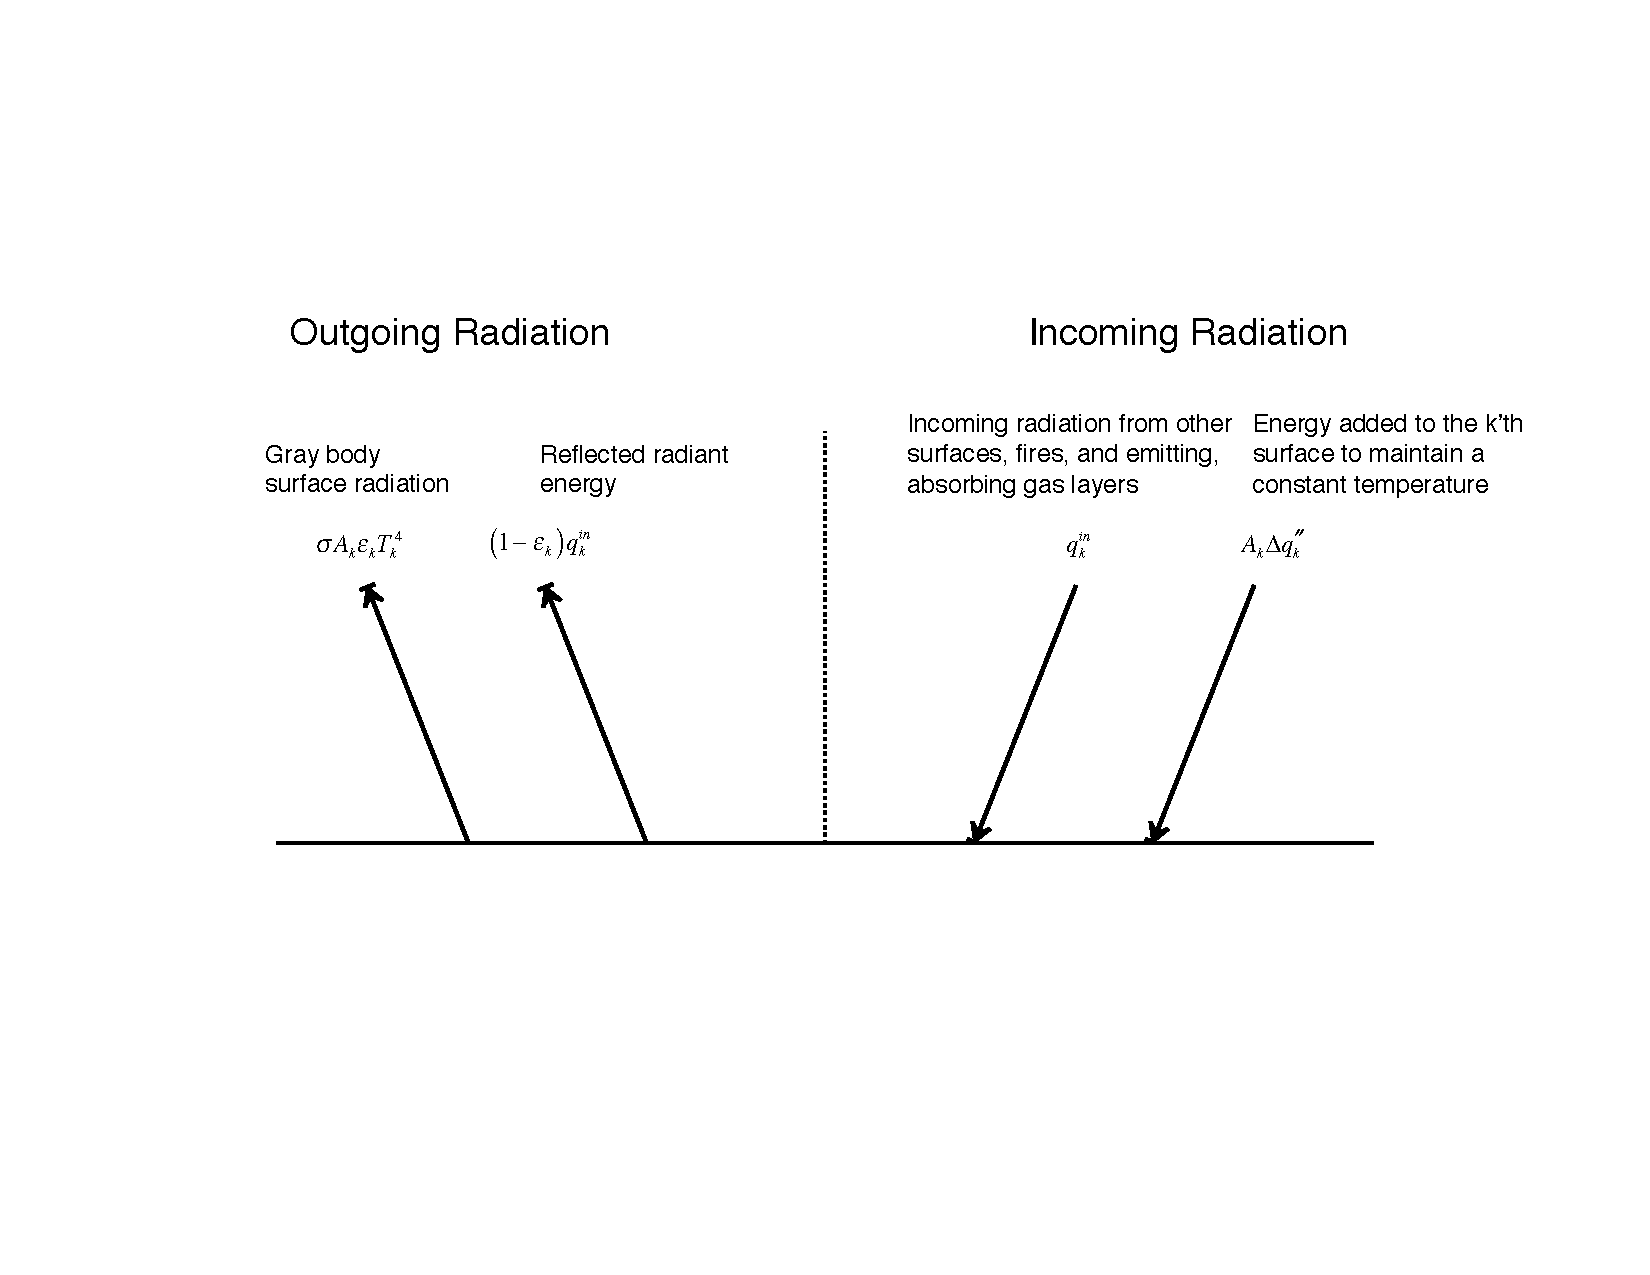
\includegraphics[width=5.0in]{FIGURES/Theory/Radiation_Exchange}\\
\end{center}
\caption{Radiation Exchange in a two-zone fire model.}
 \label{fig:Rad_Exchange}
\end{figure}

The walls can be modeled using two surfaces or four.  The four wall model is necessary for fire rooms because the temperatures of the ceiling and upper walls differ significantly.  The two wall model is used for compartments that contain no fires.

To simplify the comparison between the two and four wall segment models, assume that the emissivities of all wall segments are one and that the gas absorptivities are zero.  Let the room dimensions be 4 m ? 4 m ? 4 m, the temperature of the floor and the lower and upper walls be 300 K, and the ceiling temperature vary from 300 K to 600 K. Figure \ref{fig:Rad_2vs4} shows a plot of the heat flux to the ceiling and upper wall as a function of the ceiling temperature \cite{Forney_radiation, Jones:1993}. The two wall model predicts that the extended ceiling (a surface formed by combining the ceiling and upper wall into one wall segment) cools, while the four wall model predicts that the ceiling cools and the upper wall warms.  The four-wall model moderates temperature differences that may exist between the ceiling and upper wall (or floor and lower wall) by allowing heat transfer to occur between the ceiling and upper wall. This problem does not arise when a fire is not present.

Reference \cite{Forney_radiation} documents how to minimize the work required to compute the 16 configuration factors, $F_{k-j}$, required in a 4 wall model.

\begin{figure}
\begin{center}
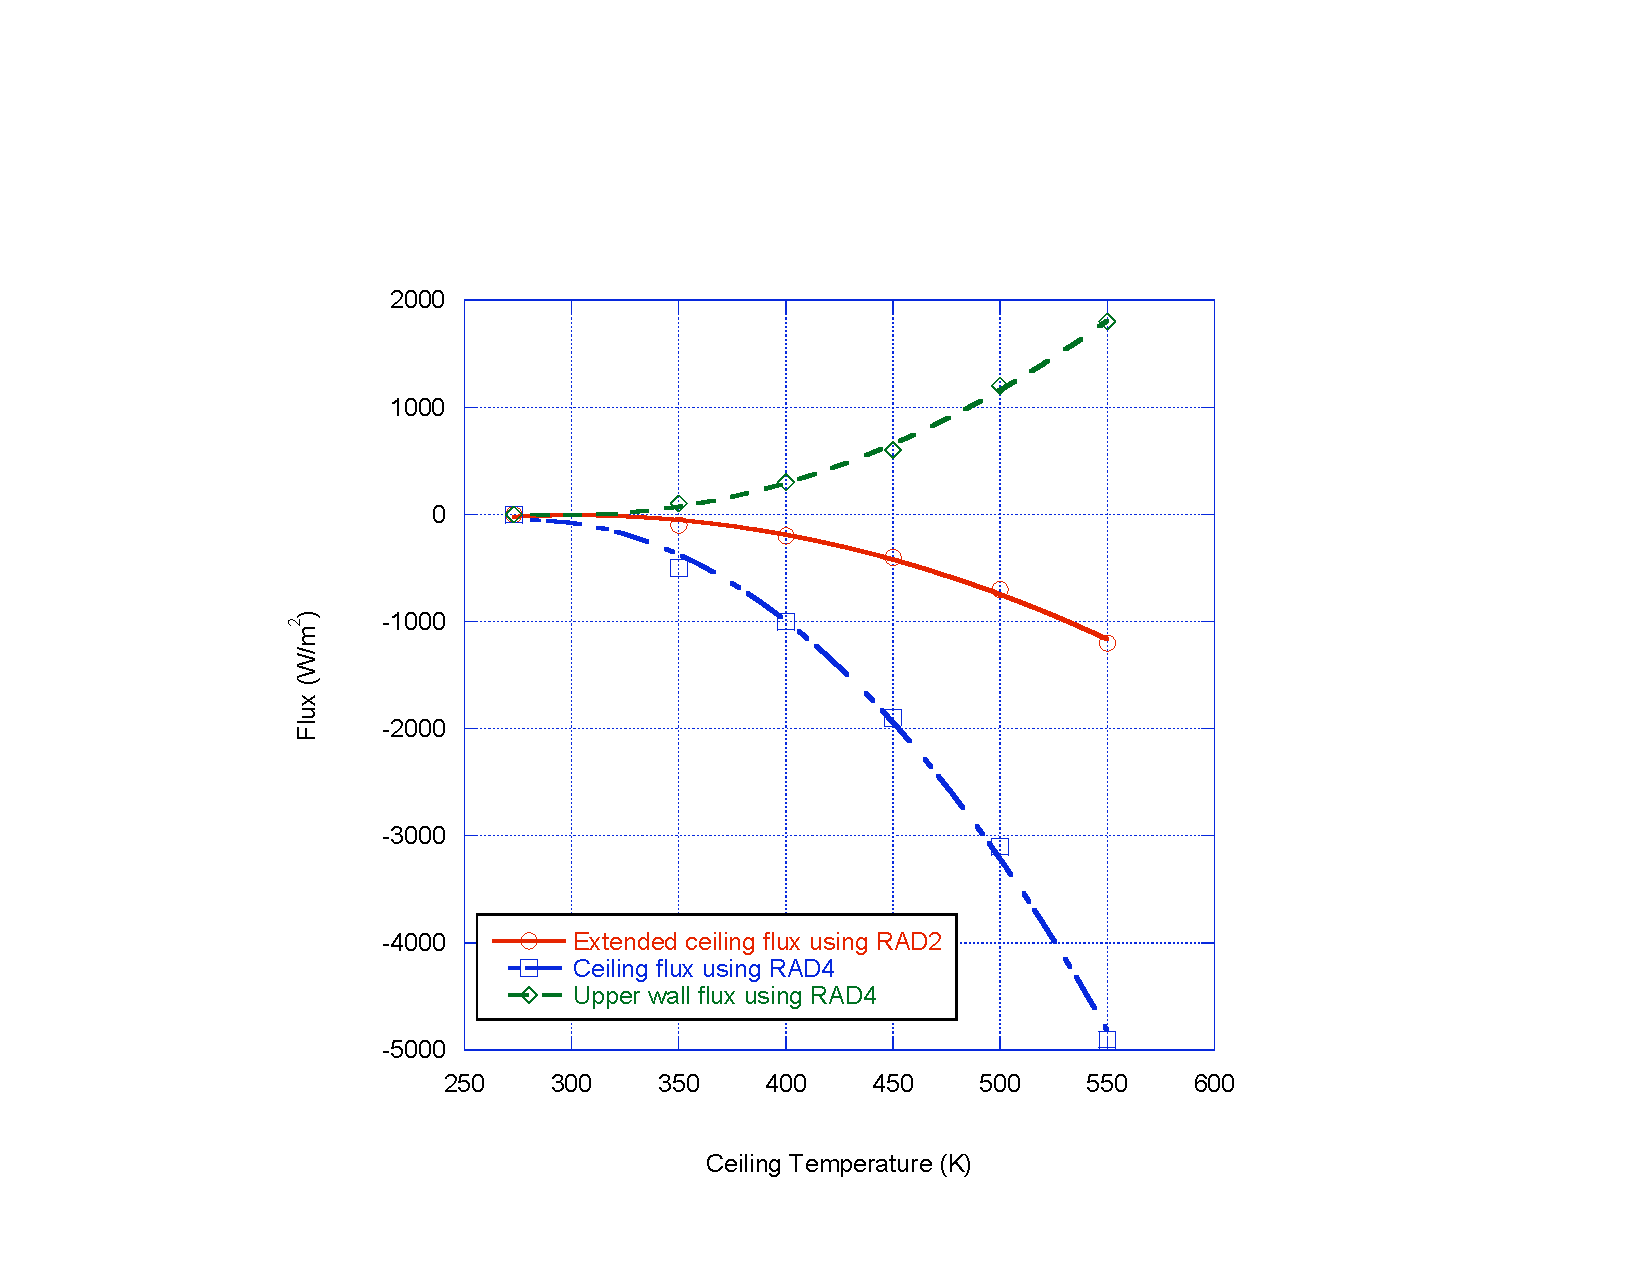
\includegraphics[width=5.0in]{FIGURES/Theory/Radiation_2vs4}\\
\end{center}
\caption{An example of the calculated two-wall (RAD2) and four-wall (RAD4) contributions to radiation exchange on a ceiling and wall surface.}
 \label{fig:Rad_2vs4}
\end{figure}

{\bf Configuration Factors:}  A configuration factor between two finite areas denoted $F_{1-2}$ is the fraction of radiant energy given off by surface 1 that is intercepted by  surface 2 and is given by

\be F_{1-2} = \frac{1}{A_1} \int_{A_1} \int_{A_2} \frac{\cos \theta_1 \theta_2}{\pi L^2} dA_1 dA_2 \label{eq:config_factor} \ee
where $L$ is the distance along the line of integration,  $\theta_1$ and $\theta_2$ are the angles for surface 1 and 2 between the respective normal vectors and the line of integration, and $A_1$ and $A_2$ are the areas of the two surfaces.  These terms are illustrated in figure \ref{fig:Rad_Config_Factor}.  When the surfaces $A_1$ and $A_2$ are far apart relative to their surface area, eq (\ref{eq:config_factor}) can be approximated by assuming that $\theta_1$, $theta_2$ and $L$ are constant over the region of integration to obtain

\begin{figure}
\begin{center}
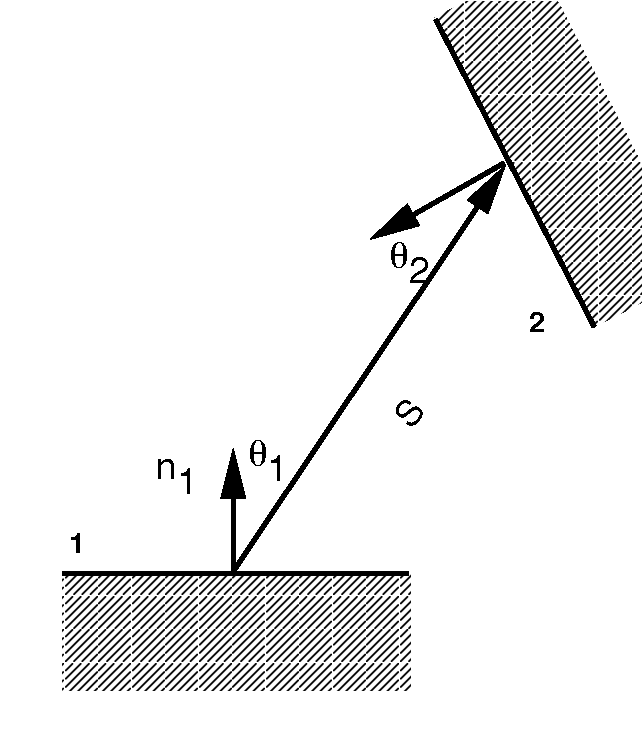
\includegraphics[width=3.0in]{FIGURES/Theory/Radiation_Config_Factor}\\
\end{center}
\caption{Setup for a configuration factor calculation between two arbitrarily oriented finite areas.}
 \label{fig:Rad_Config_Factor}
\end{figure}

\be F_{1-2} = \frac{\cos \theta_1 \theta_2}{\pi L^2} A_2 \ee

{\bf Transmittance and Absorptance:} The transmittance of a gas volume is the fraction of radiant energy that will pass through it unimpeded and is given by

\be \tau (L) = e^{-aL} \ee
where $a$ is the absorption coefficient of the gas volume and $L$ is a characteristic path length.

The absorptance, $\alpha$, of a gas volume is the fraction of radiant energy absorbed by that volume.  For a gray gas, $\alpha + \tau = 1$.

{\bf Calculating absorption for broad band gas layer radiation:}  In general, the transmittance and absorptance are a function of wavelength.   This is an important factor to consider for the major gaseous products ($\textnormal{CO}_2$  and $\textnormal{H}_2 \textnormal{O}$); however soot has a continuous absorption spectrum which allows the transmittance and absorptance to be approximated as ``gray" \cite{SiegelandHowell:1981} across the entire spectrum.

The gas absorptance, $\alpha_G$, is due to the combination of the $\textnormal{CO}_2$  and $\textnormal{H}_2 \textnormal{O}$ and is given by

\be \alpha_G = \alpha_{H_2O} + \alpha_{CO} - C\ee
where $C$ is a correction for band overlap.  For typical fire conditions, the overlap amounts to about half of the $\textnormal{CO}_2$ absorptance \cite{Tien:2002} so the gas transmittance is approximated by

\be \tau_G = 1 - \alpha_{H_2O} - 0.5 \alpha_{CO_2} \ee

The total transmittance of a gas-soot mixture is the product of the gas and soot transmittances, $\tau_T = \tau_S \tau_G$ so that

\be \tau_T = e^{-al} \brackets{1 - \alpha_{H_2O} - 0.5 \alpha_{CO_2}} \ee

In the optically thin limit the absorption coefficient, a, may be replaced by the Planck mean absorption coefficient and in the optically thick limit, it  may be replaced by the Rosseland mean absorption coefficient. For the entire range of optical thicknesses, Tien et al. \cite{Tien:2002} report that a reasonable approximation is $\alpha = k f_v T$ where $k$ is a constant that depends on the optical properties of the soot particles, $f_v$ is the soot volume fraction and $T$ is the soot temperature in Kelvin. Values of $a$, have been found to be about constant for a wide range of fuels \cite{Tien:1978}.   The soot volume fraction, $f_v$, is calculated from the soot mass, soot density and layer volume.  The soot is assumed to be in thermal equilibrium with the gas layer.

Edwards' absorptance data for $\textnormal{H}_2 \textnormal{O}$ and $\textnormal{CO}_2$ are reported \cite{Edwards:1985} as log(emissivity) versus log(pressure-pathlength), with  log(gas concentration) as a parameter. For each gas, these data were incorporated into a look-up table, implemented as a two-dimensional array of log(emissivity) values, with indices based on temperature and gas concentration.  It is assumed that absorptance and emittance are equivalent for the gaseous species as well as for soot.

An effective path length ( mean beam length, L) treats an emitting volume as if it were a hemisphere of a radius such that the flux impinging on the center of the circular base is equal to the average boundary flux produced by the real volume. The value of this radius is approximated as \cite{Tien:1978, Hottel:1942} $L = c 4 V / A$ where $L$ is the mean beam length in meters, $c$ is a constant (approximately 0.9, for typical geometries), $V$ is the emitting gas volume m$^3$ and $A$ is the surface area (m$^2$) of the gas volume. The volume and surface area are calculated from the dimensions of the layer.

For each gas, the log(absorptance) is estimated from the look-up table for that gas  by  interpolating both the log(temperature) and log(concentration) domains. In the event that the required absorptance lies outside the temperature or concentration range of the look-up table, the nearest acceptable value is returned. Error flags are also returned, indicating whether each parameter was in or out of range and, in the latter case, whether it was high or low.  This entire process is carried out for both $\textnormal{CO}_2$  and $\textnormal{H}_2 \textnormal{O}$.

\subsubsection{Computing Target Heat Flux and Temperature}

The calculation of the radiative heat flux to a target is similar to the radiative heat transfer calculation discussed previously.  The main difference is that CFAST does not compute feedback from the target to the wall surfaces or gas layers.  The target is simply a probe or sensor not interacting with the modeled environment.  

The net flux striking a target can be used as a boundary condition in order to compute the temperature of the target.  If the target is thin, then its temperature quickly rises to a level where the heat flux to and from the target are in equilibrium.

There are four components of heat flux to a target: fires, walls (including the ceiling and floor), gas layer radiation and gas layer convection.